\documentclass{article}%
\usepackage[T1]{fontenc}%
\usepackage[utf8]{inputenc}%
\usepackage{lmodern}%
\usepackage{textcomp}%
\usepackage{lastpage}%
%
\usepackage{amsmath}%
\usepackage{amssymb}%
\usepackage{amsfonts}%
\usepackage{graphicx}%
\usepackage{hyperref}%
\usepackage{tikz}%
\usepackage{pgfplots}%
\usetikzlibrary{math}%
\title{IME 2026 - Física\thanks{This exam was solved and automatically generated with gpt-resolve: \url{https://github.com/lgabs/gpt-resolve}}}%
\author{claude{-}haiku{-}5{-}5 (solver) + claude{-}haiku{-}5{-}5 (judge)}%
\date{November 10, 2026}%
%
\begin{document}%
\normalsize%
\maketitle%
\section*{Questão 1}

\section*{Solução}

\textbf{Hipóteses e relações básicas.} Partícula de massa $m$ (não fornecida; os itens (a) e (b) não dependem de $m$), movimento unidimensional sem dissipação. A força é conservativa: $F(x)=-\dfrac{dE_p}{dx}=-(4x-x^{2})=-4x+x^{2}$, como no enunciado. Pela conservação da energia mecânica,
\[
E=\tfrac12 m v^{2}+E_p(x)\quad\Longrightarrow\quad v^{2}=\frac{2}{m}\bigl[E-E_p(x)\bigr]\ge 0 .
\]
Logo o movimento ocorre em $\{x:\,E_p(x)\le E\}$, e os pontos de retorno ($v=0$) são as raízes de $E_p(x)=E$. Num retorno simples ($E_p'\neq 0$), $|v|\propto\sqrt{|x-x_r|}$ e o retorno é atingido em tempo finito. Com $x$ em metros, os coeficientes de $E_p$ são implicitamente $2\,\mathrm{J/m^{2}}$ e $\tfrac13\,\mathrm{J/m^{3}}$.

\textbf{Estrutura de $E_p$.} Temos
\[
E_p(x)=\frac{x^{2}(6-x)}{3},\qquad E_p'(x)=x(4-x),\qquad E_p(x)=\frac{32}{3}-\frac{(x-4)^{2}(x+2)}{3},
\]
a última identidade conferida por $(x-4)^{2}(x+2)=x^{3}-6x^{2}+32$. Assim:
\begin{itemize}
\item $x=0$ é mínimo ($E_p''(0)=4>0$, $E_p(0)=0$): equilíbrio estável. $x=4$ é máximo ($E_p''(4)=-4<0$, $E_p(4)=\tfrac{32}{3}\,\mathrm{J}\approx 10{,}7\,\mathrm{J}$): barreira, equilíbrio instável.
\item Pelo sinal de $E_p'=x(4-x)$: $E_p$ decresce de $+\infty$ a $0$ em $(-\infty,0]$, cresce de $0$ a $\tfrac{32}{3}$ em $[0,4]$ e decresce de $\tfrac{32}{3}$ a $-\infty$ em $[4,\infty)$. Além disso $E_p\ge 0$ para $x\le 6$, com $E_p(6)=0$.
\item $E_p(x)<\tfrac{32}{3}$ para $x>-2$, $x\neq 4$, e $E_p(x)>\tfrac{32}{3}$ para $x<-2$. Em $x=-2$ tem-se $E_p=\tfrac{32}{3}$, mas $E_p'(-2)=-12\neq 0$: não é extremo.
\end{itemize}

\textbf{a)} Oscilação é movimento periódico entre dois retornos $x_1<x_2$. Por faixas de $E$:
\begin{itemize}
\item $E<0$: a região permitida é $[x_E,\infty)$, com $x_E>6$; é ilimitada. Para $E=0$ a região é $\{0\}\cup[6,\infty)$, e $x=0$ é apenas repouso. Não há oscilação.
\item $0<E<\tfrac{32}{3}$: como $E_p(-2)=\tfrac{32}{3}>E>0=E_p(0)$, $E_p(0)=0<E<E_p(4)=\tfrac{32}{3}$ e $E_p(4)=\tfrac{32}{3}>E>0=E_p(6)$, e pelas monotonias, as raízes de $E_p=E$ são $x_L\in(-2,0)$, $x_2\in(0,4)$ e $x_3\in(4,6)$. A região permitida é $[x_L,x_2]\cup[x_3,\infty)$, com barreira em $(x_2,x_3)$. A componente limitada $[x_L,x_2]$, que contém $0$, é percorrida periodicamente, com retornos simples ($E_p'(x_L)\neq 0\neq E_p'(x_2)$) e, portanto, período finito. A componente $[x_3,\infty)$ é ilimitada: lá $F>0$ e a partícula escapa para $+\infty$.
\end{itemize}
\textit{Posições possíveis.} Uma posição $x_0$ pode oscilar se existe $E$ tal que $x_0$ pertence à componente limitada.
\begin{itemize}
\item $-2<x_0<4$: tem-se $0\le E_p(x_0)<\tfrac{32}{3}$. Escolha $E\in\bigl(E_p(x_0),\tfrac{32}{3}\bigr)$, o que dá $E>0$. No segmento entre $0$ e $x_0$, o máximo de $E_p$ é $E_p(x_0)$: se $x_0>0$, $E_p$ é crescente em $[0,x_0]$ (pois $E_p'>0$ em $(0,4)$); se $x_0<0$, $E_p$ é decrescente em $[x_0,0]$ (pois $E_p'<0$ em $(-\infty,0)$). Como $E_p(x_0)<E$, o segmento inteiro está em $\{E_p\le E\}$ e é conexo com $0$. Logo está na componente $[x_L,x_2]$, que contém $x_0$.
\item $x_0\le -2$ ou $x_0=4$: então $E\ge E_p(x_0)\ge\tfrac{32}{3}$, e não há oscilação (item b). Para $x_0>4$ e $E\le 0$ ou $0<E<\tfrac{32}{3}$, $x_0$ é proibida ou pertence a componente ilimitada; para $E\ge\tfrac{32}{3}$ não há oscilação.
\end{itemize}
\textit{Resposta:} $-2\,\mathrm{m}<x<4\,\mathrm{m}$, com $0<E<\tfrac{32}{3}\,\mathrm{J}$. Os extremos não são atingidos, pois exigiriam $E\ge\tfrac{32}{3}\,\mathrm{J}$. \textit{Conferência:} para $E\to 0^{+}$, $E_p\approx 2x^{2}=\tfrac12\cdot 4\cdot x^{2}$, logo $\omega=\sqrt{4/m}=2/\sqrt{m}$ e $T\to\pi\sqrt{m}$, como no oscilador harmônico.

\textbf{b)}
\begin{itemize}
\item $E>\tfrac{32}{3}$: em $(-\infty,0]$ há um único retorno $x_t$, com $x_t<-2$, pois $E_p(-2)=\tfrac{32}{3}<E$. Em $[0,\infty)$ tem-se $E_p\le\tfrac{32}{3}<E$, logo $v^{2}>0$ e não há retorno. A partícula é refletida em $x_t$ e, uma vez em $x\ge 0$ com $v>0$, não pode voltar. Para $x\to\infty$, $v\simeq\sqrt{2x^{3}/(3m)}$, logo $\int_4^\infty dx/v<\infty$: a fuga ocorre em tempo finito. Não há movimento periódico.
\item $E=\tfrac{32}{3}$: a região permitida é $[-2,\infty)$, com $v^{2}=\dfrac{2}{m}\cdot\dfrac{(x-4)^{2}(x+2)}{3}$ e $|v|\simeq\dfrac{2}{\sqrt{m}}|x-4|$ perto de $x=4$. Logo $\int dx/|v|$ diverge logaritmicamente e $x=4$ só é atingido em tempo infinito. Casos: (i) $x\in(-2,4)$ com $v<0$: reflete em $x=-2$ (retorno simples, tempo finito) e depois sobe monotonicamente a $4$, assintoticamente; (ii) $x\in(-2,4)$ com $v>0$: sobe a $4$ assintoticamente; (iii) $x>4$ com $v<0$: desce a $4$ assintoticamente; (iv) $x>4$ com $v>0$: escapa em tempo finito. Em nenhum caso há retorno a um ponto de retorno após excursão finita, logo não há periodicidade. ($x=4$ com $v=0$ é equilíbrio, sem movimento.)
\end{itemize}
Logo a oscilação ocorre exatamente para $0<E<\tfrac{32}{3}\,\mathrm{J}$, e
\[
E_{\text{sup}}=E_p(4)=\frac{32}{3}\,\mathrm{J}\approx 10{,}7\,\mathrm{J}.
\]
É supremo, não máximo, pois não é atingido.

\textit{Período perto de $E_{\text{sup}}$.} Seja $\delta=E_{\text{sup}}-E\to 0^{+}$ e $u=4-x$. Como $E_p=\tfrac{32}{3}-2u^{2}+\tfrac{u^{3}}{3}$, para $u$ pequeno vale $|v|\simeq\dfrac{2}{\sqrt{m}}\sqrt{u^{2}-\delta/2}$. Os termos de ordem superior ($u^{3}/3$) alteram o integrando apenas por um fator $1+O(u)$ e, perto do retorno, por quantidade limitada: afetam só a constante aditiva. O semiperíodo $x_L\to x_2$ contém uma única passagem perto de $x=4$, a que termina no retorno $x_2$, com $u_2\simeq\sqrt{\delta/2}$. Com $c>0$ fixo,
\[
t_{L\to 2}=\frac{\sqrt{m}}{2}\int_{u_2}^{c}\frac{du}{\sqrt{u^{2}-\delta/2}}+O(1)=\frac{\sqrt{m}}{2}\operatorname{arccosh}\frac{c}{\sqrt{\delta/2}}+O(1)=\frac{\sqrt{m}}{4}\ln\frac{1}{\delta}+O(1),
\]
pois $\operatorname{arccosh}z=\ln\bigl(z+\sqrt{z^{2}-1}\bigr)\simeq\ln(2z)$ para $z\to\infty$. O trecho perto de $x_L\approx -2$ tem tempo finito. Pela simetria temporal do item (c), o semiperíodo de volta tem o mesmo tempo, logo
\[
T(E)=2\,t_{L\to 2}=\frac{\sqrt{m}}{2}\ln\frac{1}{E_{\text{sup}}-E}+O(1)\longrightarrow\infty\qquad (E\to E_{\text{sup}}^{-}).
\]
Verificação numérica ($m=1$): $t_{L\to 2}-\tfrac14\ln\tfrac1\delta\to 2{,}109$ para $\delta=10^{-2},10^{-3},10^{-4}$.

\textbf{c)} Dados: $E>\tfrac{32}{3}\,\mathrm{J}$; em $t=0$, $x=0$ e $v<0$. Como $E_p(0)=0$, $v(0)=-v_0$ com $v_0=\sqrt{2E/m}$. Equações: $\dot x=v$ e $m\dot v=F(x)=x(x-4)$.
\begin{enumerate}
\item $x<0$: $F>0$, logo $v$ cresce de $-v_0$ até $0$ em $x_t<-2$, no instante $t_1$ (finito, retorno simples; $F(x_t)>0$).
\item Simetria: $m\ddot x=F(x)$ não depende explicitamente de $t$. A função $y(t)=x(2t_1-t)$ satisfaz a mesma equação, com $y(t_1)=x_t$ e $\dot y(t_1)=0$, os mesmos dados de $x$ em $t_1$. Pela unicidade, $x(2t_1-t)=x(t)$ e $v(2t_1-t)=-v(t)$. Assim, em $t_2=2t_1$ a partícula está em $x=0$ com $v=+v_0$.
\item $0<x<4$: $F<0$, e $v$ decresce de $v_0$ até $v_4=\sqrt{\tfrac{2}{m}\bigl(E-\tfrac{32}{3}\bigr)}>0$ em $x=4$ (instante $t_3$). Não há retorno, pois $v^{2}\ge\tfrac{2}{m}(E-\tfrac{32}{3})>0$.
\item $x>4$: $F>0$ e $v$ cresce sem retorno. A fuga ocorre em $t^{*}=t_3+\int_4^\infty dx/v<\infty$ (item b). Para $x$ grande, $\dot x\propto x^{3/2}$, logo $x\propto(t^{*}-t)^{-2}$ e $v\propto(t^{*}-t)^{-3}\to+\infty$.
\end{enumerate}
Conclusão: o movimento não é oscilatório. A partícula é refletida uma vez em $x_t$ e escapa para $+\infty$ em tempo finito $t^{*}$.

\textit{Gráfico $v\times t$.} Use $\dot v=F(x)/m$ e $\ddot v=F'(x)\,v/m$, com $F'(x)=2x-4$.
\begin{itemize}
\item $t=0$: $\dot v=0$ e $\ddot v=4v_0/m>0$: mínimo com tangente horizontal. $v(0)=-v_0$ é o mínimo global de $v(t)$ para $t\ge 0$, pois em $(0,t_1)$ $v$ cresce e depois $v\ge 0$.
\item $(0,t_1)$: $v$ cresce de $-v_0$ a $0$; em $t_1$, $\dot v=F(x_t)/m>0$, cruzamento ascendente do eixo.
\item $(t_1,t_2)$: $v$ cresce de $0$ a $v_0$.
\item $t_2$: $\dot v=0$ e $\ddot v=-4v_0/m<0$: máximo local $v_0$ (não global, pois para $x>6$ tem-se $v>v_0$).
\item $(t_2,t_3)$: $\dot v<0$; $v$ decresce de $v_0$ a $v_4$.
\item $t_3$: $\dot v=0$ e $\ddot v=4v_4/m>0$: mínimo local com $v_4>0$, pois a partícula não para.
\item $(t_3,t^{*})$: $\dot v>0$ e $v\to+\infty$ quando $t\to t^{*}$, com assíntota vertical.
\item A curva é antissimétrica em relação a $(t_1,0)$, pela simetria do item 2.
\end{itemize}
Qualitativamente, este gráfico vale para todo $E>\tfrac{32}{3}\,\mathrm{J}$. Quantitativamente, $v_4/v_0=\sqrt{1-\tfrac{32}{3E}}$ depende de $E$: quando $E\to E_{\text{sup}}^{+}$, $v_4\to 0$ e o tempo de passagem perto de $x=4$ cresce como $\tfrac{\sqrt{m}}{2}\ln\dfrac{1}{E-E_{\text{sup}}}$ (mesmo cálculo do item b). O vale em torno de $t_3$ torna-se então um patamar longo e próximo de $v=0$, sem atingi-lo.

\textit{Exemplo numérico} ($m=1\,\mathrm{kg}$, $E=16\,\mathrm{J}$, por integração numérica da equação de movimento): $v_0\simeq 5{,}66\,\mathrm{m/s}$, $x_t\simeq -2{,}39\,\mathrm{m}$, $t_1\simeq 0{,}64\,\mathrm{s}$, $t_2\simeq 1{,}28\,\mathrm{s}$, $t_3\simeq 2{,}19\,\mathrm{s}$, $v_4\simeq 3{,}27\,\mathrm{m/s}$, $v(3\,\mathrm{s})\simeq 12{,}6\,\mathrm{m/s}$, $t^{*}\simeq 3{,}98\,\mathrm{s}$.

\begin{center}
\begin{tikzpicture}[x=1.6cm, y=0.2cm, font=\small]
  \draw[->] (-0.2,0) -- (4.4,0) node[right] {$t\,(\mathrm{s})$};
  \draw[->] (0,-8) -- (0,38) node[above] {$v\,(\mathrm{m/s})$};
  \draw[dotted] (0,5.66) -- (1.28,5.66);
  \node[left] at (0,5.66) {$v_0$};
  \node[left] at (0,-5.66) {$-v_0$};
  \draw[dotted] (0.64,-8) -- (0.64,0);
  \draw[dotted] (1.28,-8) -- (1.28,5.66);
  \draw[dotted] (2.19,-8) -- (2.19,3.27);
  \draw[dashed] (3.98,-8) -- (3.98,38);
  \node[below] at (0.64,-8) {$t_1$};
  \node[below] at (1.28,-8) {$t_2$};
  \node[below] at (2.19,-8) {$t_3$};
  \node[below] at (3.98,-8) {$t^{*}$};
  \node[below left] at (2.19,3.27) {$v_4$};
  \draw[very thick, color=blue!70!black, smooth] plot coordinates {(0,-5.66) (0.25,-4.81) (0.5,-2.08) (0.64,0) (0.75,1.65) (1.0,4.58) (1.25,5.65) (1.28,5.66) (1.5,5.23) (1.75,4.27) (2.0,3.48) (2.19,3.27) (2.5,4.02) (2.75,6.39) (3.0,12.6) (3.25,31.1)};
  \draw[very thick, color=blue!70!black, ->] (3.25,31.1) -- (3.6,37.5);
  \node[above left] at (3.3,36) {$v\to+\infty$};
\end{tikzpicture}
\end{center}
\textit{Esboço de $v\times t$ para $E>\tfrac{32}{3}\,\mathrm{J}$, com os valores do exemplo numérico; a forma qualitativa é geral.}

ANSWER: (a) $-2\,\mathrm{m}<x<4\,\mathrm{m}$, para $0<E<\tfrac{32}{3}\,\mathrm{J}$; (b) $E_{\text{sup}}=\dfrac{32}{3}\,\mathrm{J}\approx 10{,}7\,\mathrm{J}$ (supremo não atingido; o período diverge como $\tfrac{\sqrt{m}}{2}\ln\dfrac{1}{E_{\text{sup}}-E}$); (c) $v(0)=-\sqrt{2E/m}$; a velocidade anula-se em $x_t<-2$, volta a $+\sqrt{2E/m}$ em $x=0$, decresce até $v_4>0$ em $x=4$ e cresce sem limite, com assíntota vertical, em tempo finito; não há oscilação.%
\newpage%
\section*{Questão 2}

\section*{Solução}

\noindent\textbf{Hipóteses e notação.} (i) A e B têm órbitas circulares em torno da mesma estrela S; logo ambos obedecem à 3ª lei de Kepler com a mesma constante $GM_S$. (ii) Como $R \ll r$, a distância de S a cada corpo é o raio orbital $r$, e a distância de um ponto da superfície ao centro do planeta é $R$. (iii) Dimensões iguais: $R_A = R_B = R_{CA} = R$. (iv) O choque é instantâneo, de modo que o impulso da gravidade de S durante o choque é desprezível e vale a conservação do momento linear; "perfeitamente inelástico" significa que os corpos se unem, $M_{CA} = M_A + M_C$. (v) A colisão é frontal, com A e C em sentidos opostos, logo as velocidades são colineares. A velocidade de A é tangente à sua órbita circular; portanto a de C e, pela conservação do momento, a de CA também são tangentes. Assim, o ponto do choque (distância $r_A$ de S) é um apsis da órbita de CA. (vi) Energia mecânica $E = \frac{1}{2}Mv^2 - \frac{GM_SM}{r}$, com potencial nulo no infinito.

\noindent\textbf{a) Razão entre os raios.} Em dias terrestres, $T_A = 160\cdot 4 = 640$ e $T_B = 90\cdot 3 = 270$. Pela 3ª lei de Kepler,
\[
\left(\frac{r_A}{r_B}\right)^3 = \left(\frac{T_A}{T_B}\right)^2 = \left(\frac{64}{27}\right)^2 = \left(\frac{4}{3}\right)^6 \quad\Rightarrow\quad \frac{r_A}{r_B} = \left(\frac{4}{3}\right)^2 = \frac{16}{9} \approx 1{,}78.
\]

\noindent\textbf{b) Razão entre as velocidades orbitais.} Em órbita circular, $v = \frac{2\pi r}{T}$, logo
\[
\frac{v_A}{v_B} = \frac{r_A}{r_B}\cdot\frac{T_B}{T_A} = \frac{16}{9}\cdot\frac{27}{64} = \frac{3}{4} = 0{,}75.
\]
Conferência: $v = \sqrt{GM_S/r}$ dá $v_A/v_B = \sqrt{r_B/r_A} = \sqrt{9/16} = 3/4$. A é mais lento, como deve ser por estar mais afastado.

\noindent\textbf{c) Razão entre as massas de B e CA.} Um corpo de massa $m$ na superfície de um corpo de massa $M$ e raio $R$ sofre de S a força $GM_Sm/r^2$ e do próprio corpo a força $GMm/R^2$. Logo
\[
\frac{F_S}{F_{\text{corpo}}} = \frac{M_S}{M}\left(\frac{R}{r}\right)^2.
\]
Para B, $2{,}048\% = 0{,}02048$:
\[
\frac{M_S}{M_B}\left(\frac{R}{r_B}\right)^2 = 0{,}02048. \qquad (1)
\]
Para CA, logo após o choque, a distância a S é $r_A$ (CA ocupa o ponto de colisão, sobre a órbita de A) e o raio é $R$. Com $0{,}081\% = 0{,}00081$:
\[
\frac{M_S}{M_{CA}}\left(\frac{R}{r_A}\right)^2 = 0{,}00081. \qquad (2)
\]
Dividindo (2) por (1), $M_S$ e $R$ se cancelam:
\[
\frac{M_B}{M_{CA}}\left(\frac{r_B}{r_A}\right)^2 = \frac{0{,}00081}{0{,}02048} = \frac{81}{2048}
\quad\Rightarrow\quad
\frac{M_B}{M_{CA}} = \frac{81}{2048}\cdot\frac{256}{81} = \frac{1}{8} = 0{,}125.
\]
Logo $M_{CA} = 8M_B$. Como os raios são iguais, a densidade média de CA é oito vezes a de B.

\noindent\textbf{d) Razão entre $v_B$ e $v_{CA}$ logo após o choque.} Para B em órbita circular, $v_B^2 = GM_S/r_B$, logo
\[
E_B = \frac{1}{2}M_Bv_B^2 - \frac{GM_SM_B}{r_B} = -\frac{1}{2}M_Bv_B^2 < 0.
\]
Para CA logo após o choque, na posição $r_A$ e com velocidade $v_{CA}$,
\[
E_{CA} = \frac{1}{2}M_{CA}v_{CA}^2 - \frac{GM_SM_{CA}}{r_A}.
\]
A condição $E_{CA} = 7E_B$, com $M_B = M_{CA}/8$, fornece
\[
\frac{1}{2}M_{CA}v_{CA}^2 - \frac{GM_SM_{CA}}{r_A} = -\frac{7}{16}M_{CA}v_B^2.
\]
Dividindo por $M_{CA}$ e usando $\frac{GM_S}{r_A} = \frac{r_B}{r_A}v_B^2 = \frac{9}{16}v_B^2$:
\[
\frac{1}{2}v_{CA}^2 = \frac{9}{16}v_B^2 - \frac{7}{16}v_B^2 = \frac{1}{8}v_B^2 \quad\Rightarrow\quad v_{CA} = \frac{v_B}{2} \quad\Rightarrow\quad \frac{v_B}{v_{CA}} = 2.
\]
Observe que $E_{CA}$ depende apenas de $M_{CA}$, de modo que não é preciso separar $M_A$ e $M_C$.

\noindent\textbf{e) Apoastro ou periastro?} O ponto do choque está a $r_A$ de S e a velocidade é tangente, logo esse ponto é um apsis. Pela equação vis-viva, $v^2 = GM_S\left(\frac{2}{r} - \frac{1}{a}\right)$. Como $v_{CA}^2 = \frac{v_B^2}{4} = \frac{GM_S}{4r_B} = \frac{4}{9}\cdot\frac{GM_S}{r_A}$,
\[
\frac{1}{a} = \frac{2}{r_A} - \frac{4}{9r_A} = \frac{14}{9r_A} \quad\Rightarrow\quad a = \frac{9}{14}r_A < r_A.
\]
No periastro, $r_p = a(1-e) \le a$; logo um ponto com $r = r_A > a$ só pode ser o apoastro. Verificação: $v_{CA} = \frac{v_B}{2} < \sqrt{\frac{GM_S}{r_A}} = \frac{3}{4}v_B$, ou seja, a velocidade é menor que a circular nesse raio, o que caracteriza o apoastro. Pela conservação do momento angular, $h = r_Av_{CA} = \sqrt{GM_Sa(1-e^2)}$, o que dá $e^2 = \frac{25}{81}$, isto é, $e = \frac{5}{9}$. Então $r_A = a(1+e)$ (apoastro) e $r_p = a(1-e) = \frac{2}{7}r_A > 0$.

\noindent\textbf{Conferências.} As razões são adimensionais. As energias são negativas e $|E_{CA}| = 7|E_B|$. A 3ª lei de Kepler é satisfeita, pois $(T_A/T_B)^{2/3} = (64/27)^{2/3} = 16/9$. Por fim, $v_A/v_B = \sqrt{r_B/r_A}$, como exige a órbita circular em torno da mesma estrela.

ANSWER: a) $r_A/r_B = 16/9$ (aprox. 1,78); b) $v_A/v_B = 3/4$ (0,75); c) $M_B/M_{CA} = 1/8$ (0,125); d) $v_B/v_{CA} = 2$; e) apoastro, pois $v_{CA} = v_B/2 < v_{\text{circ}}(r_A) = 3v_B/4$ e $r_A > a = 9r_A/14$.%
\newpage%
\section*{Questão 3}

\section*{Solução}

\textbf{Hipóteses e modelagem.} Esfera puntiforme de massa $m$; fio ideal (inextensível, de massa desprezível), que só traciona ao longo de si ($T\ge 0$) e não exerce força quando está frouxo; sem atrito nem resistência do ar; $g$ constante; $0<d<\ell$, para que a esfera passe abaixo de $B$. Como idealização do enunciado, a barra atua apenas como pivô: após o encontro, o fio gira em torno de $B$ e a barra não entra no cálculo da trajetória. Referencial na origem em $A$, com $y$ vertical para cima. Usaremos a energia por unidade de massa $\varepsilon=\dfrac{v^2}{2}+gy$, que é nula no instante inicial (repouso em $y=0$).

\textbf{1. Descida em torno de $A$.} Durante o arco de centro $A$, a tração é radial e a velocidade é tangencial: a tração não realiza trabalho e $\varepsilon$ se conserva. Do repouso na horizontal até o ponto mais baixo ($y=-\ell$):
\[
\frac{v_0^2}{2}=g\ell\quad\Rightarrow\quad v_0^2=2g\ell .
\]
Medindo $\alpha$ a partir da vertical para baixo, $v^2=2g\ell\cos\alpha$ e, pela direção radial, $T=3mg\cos\alpha\ge 0$ para $0\le\alpha\le\dfrac{\pi}{2}$. Logo o fio permanece esticado.

\textbf{2. O fio se prende em $B$.} O fio encosta na barra quando fica vertical e passa por $B$. A esfera está então em $(0,-\ell)$, à distância $R=\ell-d$ abaixo de $B$, e o trecho livre do fio tem comprimento $R$. A velocidade é horizontal, logo já é tangente ao novo círculo de centro $B$ e raio $R$: não há componente radial a eliminar, portanto não há impulso e nenhuma energia é dissipada. Assim $v_1^2=2g\ell$, e a esfera parte do ponto mais baixo desse círculo.

\textbf{3. Movimento circular em torno de $B$.} Seja $\vec r=R(\cos\varphi,\ \sin\varphi)$ a posição relativa a $B$, com $\varphi=-\dfrac{\pi}{2}$ no ponto mais baixo. A subida pelo lado esquerdo corresponde a $\varphi$ decrescendo de $-\dfrac{\pi}{2}$ até $-\pi$ (ponto mais à esquerda) e até $-\dfrac{3\pi}{2}$ (topo). Nesse trecho $\sin\varphi$ cresce monotonicamente de $-1$ a $+1$. Como $y=-d+R\sin\varphi$, a conservação de $\varepsilon=0$ dá
\[
v^2=2g\,(d-R\sin\varphi).
\]
Na direção radial, orientada para $B$, o peso contribui com $mg\sin\varphi$. Logo $T+mg\sin\varphi=\dfrac{mv^2}{R}$, e
\[
T=\frac{mg}{R}\left(2d-3R\sin\varphi\right).
\]
O fio permanece esticado enquanto $T\ge 0$, ou seja,
\[
\sin\varphi\le k\equiv\frac{2d}{3R}=\frac{2d}{3(\ell-d)} .
\]

\textbf{a)} Como $T$ decresce com $\sin\varphi$ e este atinge o máximo $+1$ no topo, a condição mais severa é a do topo. A semicircunferência completa exige $k\ge 1$:
\[
\frac{2d}{3(\ell-d)}\ge 1\quad\Rightarrow\quad 5d\ge 3\ell\quad\Rightarrow\quad d\ge\frac{3}{5}\,\ell .
\]
Com $d<\ell$, o intervalo válido é $\dfrac{3}{5}\ell\le d<\ell$. Conferência: para $d=\dfrac{3}{5}\ell$, $R=\dfrac{2}{5}\ell$ e $v_{\text{topo}}^2=2g(d-R)=\dfrac{2}{5}g\ell=gR$, isto é, $T=0$ exatamente no topo.

Observação: para $d\ge\dfrac{\ell}{2}$ o topo do semicírculo, no ponto $(0,\ell-2d)$ relativo a $A$, cairia sobre o trecho da barra. A resposta vale na idealização adotada, em que a barra só fixa o pivô $B$.

\textbf{b)} Para $d=\dfrac{3}{7}\ell$: $R=\dfrac{4}{7}\ell$ e $k=\dfrac{6/7}{12/7}=\dfrac{1}{2}<1$. Como $d<\dfrac{3}{5}\ell$, o fio fica frouxo antes do topo, no primeiro ponto da subida com $\sin\varphi=\dfrac{1}{2}$, isto é, $\varphi_s=-\dfrac{7\pi}{6}$ ($150^\circ$ no quadrante superior esquerdo). Nesse ponto $T=0$, e, relativo a $B$,
\[
\vec r_s=\frac{4\ell}{7}\left(-\frac{\sqrt3}{2},\ \frac12\right)=\left(-\frac{2\sqrt3}{7}\,\ell,\ \frac{2}{7}\,\ell\right),\qquad v_s^2=2g\left(d-\frac{R}{2}\right)=\frac{2}{7}\,g\ell .
\]
A velocidade é tangente ao círculo, no sentido de $\varphi$ decrescente: $\vec v_s=v_s\left(\dfrac12,\ \dfrac{\sqrt3}{2}\right)$.

Após $s$ o fio fica frouxo e a esfera sofre apenas o peso (lançamento oblíquo). Com $x_s$ e $y_s$ as coordenadas de $\vec r_s$,
\[
x(t)=x_s+\frac{v_s}{2}\,t,\qquad y(t)=y_s+\frac{\sqrt3}{2}\,v_s\,t-\frac{g}{2}\,t^2 .
\]
Para verificar que o fio continua frouxo, use $\vec r_s\cdot\vec u=\dfrac12(x_s+\sqrt3\,y_s)=0$, com $\vec u=\left(\dfrac12,\dfrac{\sqrt3}{2}\right)$, além de $|\vec r_s|=R$ e $v_s^2=g\,y_s$. Então
\[
|\vec r|^2-R^2=-g\,y_s\,t^2+v_s^2t^2-\frac{\sqrt3}{2}\,g\,v_s\,t^3+\frac{g^2}{4}\,t^4=\frac{g\,t^3}{4}\left(g\,t-2\sqrt3\,v_s\right).
\]
Essa expressão é negativa para $0<t<t_*=\dfrac{2\sqrt3\,v_s}{g}$, de modo que o fio segue frouxo. Antes de $t_*$ a esfera está em $x<0$, longe da barra, que está em $x=0$ acima de $B$. Em $t_*$:
\[
x(t_*)=x_s+\frac{\sqrt3\,v_s^2}{g}=0,\qquad y(t_*)=y_s-\frac{3v_s^2}{g}=-2y_s=-R .
\]
Ou seja, o fio volta a esticar no ponto $(0,-R)$ relativo a $B$, isto é, abaixo de $B$.

\textbf{Retensionamento.} Nesse ponto $v_x=\dfrac{v_s}{2}$ (tangencial) e $v_y=-\dfrac{3\sqrt3}{2}v_s$ (radial, para fora). O fio, inextensível, aplica um impulso radial que anula $v_y$ e conserva $v_x$. A energia cinética cai para $\dfrac{1}{2}\cdot\dfrac{v_s^2}{4}=\dfrac{g\ell}{28}$, e $\varepsilon=\dfrac{g\ell}{28}-g\ell=-\dfrac{27}{28}\,g\ell$. Depois disso a esfera oscila como pêndulo de comprimento $R$ em torno de $B$, com $R(1-\cos\theta_{\max})=\dfrac{\ell}{28}$, ou seja, $\cos\theta_{\max}=\dfrac{15}{16}$ ($\theta_{\max}\approx 20{,}4^\circ$). Sua tração $T=m\left(\dfrac{v^2}{R}+g\cos\theta\right)$ é positiva, de modo que o fio segue esticado e a esfera nunca sobe acima de $y=-\dfrac{27}{28}\,\ell$ relativo a $A$, que está abaixo de $B$.

\textbf{Ponto mais alto após $B$.} Comparando os trechos (coordenadas relativas a $A$):
\begin{itemize}
\item arco de $\varphi=-\dfrac{\pi}{2}$ até $\varphi_s$: $y$ cresce até $y_s-d=-\dfrac{\ell}{7}$;
\item lançamento oblíquo de $s$ até $(0,-R)$: $y$ é máximo onde $v_y=0$, isto é, em $t_V=\dfrac{\sqrt3\,v_s}{2g}=\dfrac{t_*}{4}$, com $x_V=-\dfrac{3\sqrt3}{14}\,\ell$ e $y_V=y_s+\dfrac{3v_s^2}{8g}=\dfrac{11}{28}\,\ell$ relativo a $B$, ou seja, $y_V=-\dfrac{\ell}{28}$ relativo a $A$;
\item pêndulo final: $y\le -\dfrac{27}{28}\,\ell$.
\end{itemize}
Logo o apogeu $V$ é o ponto mais alto de toda a trajetória após passar por $B$.

No apogeu a velocidade é horizontal, $v_V=\dfrac{v_s}{2}$, e a aceleração $g$ é vertical, logo é inteiramente normal à trajetória. Assim
\[
\rho=\frac{v_V^2}{g}=\frac{v_s^2}{4g}=\frac{2g\ell/7}{4g}=\frac{\ell}{14}.
\]

\textbf{Verificações.} $v^2/g$ tem dimensão de comprimento. No apogeu, $\varepsilon=\dfrac{g\ell}{28}-\dfrac{g\ell}{28}=0$, igual à energia inicial, como deve ocorrer num trecho sem perdas. A distância ao pivô no apogeu é $|\vec r_V|^2=\dfrac{27}{196}\ell^2+\dfrac{121}{784}\ell^2=\dfrac{229}{784}\ell^2<\dfrac{256}{784}\ell^2=R^2$, o que confirma que o fio está frouxo. No limite $d\to\dfrac{3}{5}\ell$ do item (a), o ponto de folga migra para o topo, onde $T=0$, em acordo com a análise.

ANSWER: a) $d_{\min}=\dfrac{3}{5}\,\ell$ (válido para $\dfrac{3}{5}\ell\le d<\ell$); b) $\rho=\dfrac{\ell}{14}$%
\newpage%
\section*{Questão 4}

\section*{Solução}

\textbf{Hipóteses e topologia.} Fontes, chaves e fios são ideais. Todos os elementos são resistivos (não há capacitores nem indutores): não há transitório, cada fechamento altera as correntes instantaneamente e a potência é constante entre os instantes de chaveamento. Pela figura, as três baterias têm a mesma orientação (polo positivo, placa longa, voltado para o fio superior), logo cada ramo tem FEM $V$. Ramos em paralelo com a mesma FEM não somam tensão: a tensão em circuito aberto continua $V$, e o que se soma são as correntes. Como as FEMs são iguais, não circula corrente entre os ramos. Uma bateria invertida alteraria a FEM equivalente, o que não ocorre aqui.

Na figura, as chaves estão no fio superior, entre ramos consecutivos (ramos 1, 2, 3 da esquerda para a direita): $S_2$ liga os ramos 1 e 2, $S_1$ liga os ramos 2 e 3, e $S_0$ liga o ramo 3 ao nó $N_0$. Ramos sem caminho por chaves fechadas até $N_0$ têm uma extremidade flutuante e não conduzem. Como nenhuma chave reabre, o número de ramos ativos é $k=1$ em $0\le t<20\,\text{s}$, $k=2$ em $20\,\text{s}\le t<40\,\text{s}$ e $k=3$ em $40\,\text{s}\le t\le 60\,\text{s}$.

Logo após $S_0$, a figura mostra um $R_2$ em série e só depois a primeira derivação $R_2$. Portanto $N_0$ não tem derivação, e a malha é a sequência série, derivação, série, derivação, indefinidamente.

\textbf{1) Resistência de entrada da malha.} Seja $X$ a resistência entre $N_0$ e o trilho inferior, vista para a direita. Trunque a malha em $n$ seções (cada uma: $R_2$ em série seguido de $R_2$ em derivação no nó seguinte), com extremidade final aberta, e seja $X_n$ a resistência de entrada. Então $X_1=2R_2$. Para $n\ge 2$, a derivação de $N_1$ fica em paralelo com o restante da malha a partir de $N_1$, que tem $n-1$ seções e resistência de entrada $X_{n-1}$:
\[
X_n = T(X_{n-1}), \qquad T(x)=R_2+\frac{R_2\,x}{R_2+x}.
\]
A resistência da malha infinita é $X=\lim_{n\to\infty}X_n$.

\textit{Ponto fixo.} Se o limite existe, $X=T(X)$. Multiplicando por $R_2+X$ e simplificando:
\[
X^2-R_2X-R_2^2=0 \quad\Rightarrow\quad X=\frac{1\pm\sqrt{5}}{2}\,R_2 .
\]
A raiz negativa, $\frac{1-\sqrt{5}}{2}R_2=-(3-\sqrt{5})\approx -0{,}764\,\Omega$, é excluída: uma rede passiva absorve potência $I^2X\ge 0$ para toda corrente, logo $X\ge 0$. A raiz positiva é
\[
X=\frac{1+\sqrt{5}}{2}(\sqrt{5}-1)\,\Omega=\frac{5-1}{2}\,\Omega=2\,\Omega .
\]

\textit{Convergência.} $T$ é crescente para $x\ge 0$, pois $T'(x)=R_2^2/(R_2+x)^2>0$. Além disso, $X_2=\frac{5}{3}R_2\approx 2{,}06\,\Omega<X_1=2R_2\approx 2{,}47\,\Omega$; por indução, $X_{n+1}=T(X_n)<T(X_{n-1})=X_n$, logo a sequência é decrescente. Também $T(2)=2$ e $X_1>2$ (pois $2\sqrt{5}-2>2$); por indução, se $X_n>2$ então $X_{n+1}=T(X_n)>T(2)=2$, logo $X_n>2$ para todo $n$. A sequência decrescente e limitada inferiormente converge a um $L\ge 2$, e por continuidade $L=T(L)$. Pelo ponto fixo, $L=2\,\Omega$. Assim $X=2\,\Omega$, e a convergência é rápida: $X_5\approx 2{,}0002\,\Omega$.

\textit{Nota.} Se houvesse derivação em $N_0$, a resistência seria $R_2\parallel 2\,\Omega=3-\sqrt{5}\approx 0{,}764\,\Omega$, com $E\approx 5460\,\text{J}$. A figura não tem essa derivação.

\textbf{2) Equivalente de Thevenin das fontes.} Vistos de $N_0$, os $k$ ramos idênticos estão entre os mesmos nós. Em circuito aberto a tensão é $V$ (não há corrente nos ramos), e as $k$ resistências $R_1$ estão em paralelo. Logo $V_{th}=V$ e $R_{th}=R_1/k$. Como a malha é um bipolo linear, o teorema de Thevenin pode ser aplicado.

\textbf{3) Corrente e potência.} Com a malha como carga de resistência $X$:
\[
I_k=\frac{V}{R_1/k+X}, \qquad U_k=I_kX, \qquad P_k=U_kI_k=I_k^{2}X .
\]
A malha não tem fontes internas e é puramente resistiva; logo toda a potência que entra por seus terminais é dissipada nela.

\begin{center}
\begin{tabular}{c c c c c c}
Intervalo & $k$ & $R_{th}=R_1/k$ & $I_k$ & $P_k$ & $E_k=P_k\,\Delta t$ \\
\hline
$0\le t<20\,\text{s}$ & 1 & $6\,\Omega$ & $5\,\text{A}$ & $50\,\text{W}$ & $1000\,\text{J}$ \\
$20\,\text{s}\le t<40\,\text{s}$ & 2 & $3\,\Omega$ & $8\,\text{A}$ & $128\,\text{W}$ & $2560\,\text{J}$ \\
$40\,\text{s}\le t\le 60\,\text{s}$ & 3 & $2\,\Omega$ & $10\,\text{A}$ & $200\,\text{W}$ & $4000\,\text{J}$ \\
\end{tabular}
\end{center}

Por exemplo, para $k=2$: $I_2=40/(3+2)=8\,\text{A}$ e $P_2=8^2\cdot 2=128\,\text{W}$.

\textbf{4) Energia.} Como $P$ é constante em cada intervalo, $E=\sum_k P_k\,\Delta t_k$:
\[
E=20\,\text{s}\,(50+128+200)\,\text{W}=7560\,\text{J}\approx 7{,}56\,\text{kJ}.
\]

\textbf{5) Verificações.}
\begin{itemize}
\item Unidades: $\text{V}/\Omega=\text{A}$, $\text{A}^2\cdot\Omega=\text{W}$ e $\text{W}\cdot\text{s}=\text{J}$.
\item Balanço de potência (fontes = $R_1$ + malha, em W): $k=1$: $40\cdot 5=200=5^2\cdot 6+50$; $k=2$: $40\cdot 8=320=2\cdot 4^2\cdot 6+128$; $k=3$: $40\cdot 10=400=3\cdot(10/3)^2\cdot 6+200$. Todos fecham.
\item Caso particular: para $k=3$, $R_{th}=X=2\,\Omega$, logo a potência na malha é máxima (máxima transferência): $P_{\max}=V^2/(4X)=1600/8=200\,\text{W}$, o valor obtido.
\item Conferência numérica independente: análise nodal de Kirchhoff de uma escada truncada com 400 seções e extremidade aberta (sistema tridiagonal), para $k=1,2,3$, reproduz $I=5, 8, 10\,\text{A}$, $P=50, 128, 200\,\text{W}$ e $E=7560\,\text{J}$.
\end{itemize}

ANSWER: 7560 J (7,56 kJ)%
\newpage%
\section*{Questão 5}

\section*{Solução}

\textbf{Referencial e geometria.} Eixo $x$ ao longo da viga, origem em $C$, sentido para a direita. Como $CD=6$ m, $DE=4$ m e $GE=2$ m, tem-se $C:\ x=0$, $D:\ x=6$ m, $G:\ x=8$ m e $E:\ x=10$ m. O bloco está a 1 m de $E$, em $x=9$ m. Forças verticais são positivas para cima e momentos são positivos no sentido anti-horário.

\textbf{Cargas.} A viga é homogênea, com peso linear $\lambda=\dfrac{Mg}{L}=\dfrac{60\ \text{N}}{10\ \text{m}}=6$ N/m (peso por metro, equivalente a massa linear de 0,6 kg/m). Cada trecho pesa $\lambda\,\ell$ e atua no seu centro:
\begin{itemize}
\item trecho $CG$ (8 m): $48$ N em $x=4$ m;
\item trecho $GE$ (2 m): $12$ N em $x=9$ m;
\item bloco: $P=mg=10m$ N em $x=9$ m.
\end{itemize}

\textbf{Hipóteses e leis.}
\begin{itemize}
\item A viga é indeformável. Em repouso, cada parte isolada é um corpo rígido em equilíbrio: $\sum F=0$ e $\sum M=0$.
\item A distância de 1 m refere-se ao ponto de aplicação do peso do bloco (seu centro). Como as dimensões do bloco não são dadas, seu peso é tratado como força concentrada em $x=9$ m.
\item Os apoios simples $C$, $D$ e $E$ reagem apenas na vertical e só empurram: $R\geq 0$. Essa é a condição de validade do modelo.
\item A articulação em $G$ transmite força $(H_G,R_G)$ a $GE$, mas não transmite momento. Pela 3ª lei de Newton, $CG$ recebe $(-H_G,-R_G)$.
\item O dente sustenta $GE$ por baixo, isto é, só empurra: $R_G\geq 0$.
\item Não há carga horizontal e $E$ reage só na vertical. Logo $\sum F_x=0$ em $GE$ dá $H_G=0$.
\end{itemize}

\textbf{Determinação do problema.} Sem a articulação, a viga inteira tem 3 incógnitas verticais ($R_C,R_D,R_E$) e apenas 2 equações úteis ($\sum F_y=0$ e $\sum M=0$; a equação horizontal é identicamente satisfeita). Ela é hiperestática de grau 1. Com a articulação, as incógnitas são $R_C,R_D,R_E,R_G,H_G$, isto é, 5. As equações são 3 por trecho ($\sum F_x$, $\sum F_y$, $\sum M$), totalizando 6. As duas equações $\sum F_x$ coincidem ($-H_G=0$ e $H_G=0$), restando 5 independentes. O sistema é determinado e triangular: $GE$ fornece $R_G$ e $R_E$; $CG$ fornece $R_D$ e $R_C$.

\textbf{a) Para $m=4$ kg ($P=40$ N).}

Trecho $GE$: para cima, $R_G$ em $x=8$ m e $R_E$ em $x=10$ m; para baixo, $12$ N e $40$ N em $x=9$ m. Os momentos em relação a $E$ eliminam $R_E$:
\begin{align*}
\sum M_E=0:\quad 2R_G &= (12+40)\cdot 1 \Rightarrow R_G=26\ \text{N}\\
\sum F_y=0:\quad R_E &= 52-26 = 26\ \text{N}
\end{align*}

Trecho $CG$: para cima, $R_C$ em $x=0$ e $R_D$ em $x=6$ m; para baixo, $48$ N em $x=4$ m e $R_G=26$ N em $x=8$ m. Os momentos em relação a $C$ eliminam $R_C$:
\begin{align*}
\sum M_C=0:\quad 6R_D &= 48\cdot 4+26\cdot 8 = 400 \Rightarrow R_D=\frac{200}{3}\ \text{N}\approx 66{,}7\ \text{N}\\
\sum F_y=0:\quad R_C &= 48+26-\frac{200}{3}=\frac{22}{3}\ \text{N}\approx 7{,}3\ \text{N}
\end{align*}

Com $H_G=0$, as reações são $R_C=\frac{22}{3}$ N, $R_D=\frac{200}{3}$ N, $R_E=26$ N e $R_G=26$ N.

\emph{Conferências.} A soma vertical da viga inteira dá $R_C+R_D+R_E=\frac{22}{3}+\frac{200}{3}+26=100$ N $=(M+m)g$. O momento global em relação a $C$ dá $6R_D+10R_E=400+260=660$ N$\cdot$m $=60\cdot 5+40\cdot 9$ N$\cdot$m. Esta última é apenas uma conferência aritmética, pois é combinação das equações anteriores. Todas as reações são positivas, logo são compatíveis com apoios simples.

\textbf{b) Maior valor de $m$.}

Com $P=10m$ N, as mesmas equações dão:
\begin{align*}
GE\ (\textstyle\sum M_E=0):\quad 2R_G &= (12+10m)\cdot 1 \Rightarrow R_G=6+5m\ \text{N}\\
GE\ (\textstyle\sum F_y=0):\quad R_E &= 12+10m-R_G = 6+5m\ \text{N}\\
CG\ (\textstyle\sum M_C=0):\quad 6R_D &= 48\cdot 4+8R_G \Rightarrow R_D=40+\frac{20}{3}m\ \text{N}\\
CG\ (\textstyle\sum F_y=0):\quad R_C &= 48+R_G-R_D = 14-\frac{5}{3}m\ \text{N}
\end{align*}

Equivalentemente, $\sum M_D(CG)=0$ dá $6R_C=48\cdot 2-2R_G=84-10m$, a mesma expressão de $R_C$. Essa forma será usada no argumento abaixo.

\emph{Condições de validade.}
\begin{itemize}
\item \textbf{Articulação.} $R_G=6+5m>0$ para todo $m\geq 0$. O dente nunca precisa puxar $GE$, e o enunciado não fornece sua capacidade. Portanto a articulação não limita o problema. Se existisse um limite $F_{\max}$, valeria a condição extra $6+5m\leq F_{\max}$.
\item \textbf{Apoio $C$ em contato.} $R_C\geq 0 \Leftrightarrow 14-\frac{5}{3}m\geq 0 \Leftrightarrow m\leq \frac{42}{5}=8{,}4$ kg.
\item \textbf{Para $m>8{,}4$ kg não há equilíbrio.} Com $C$ em contato, $R_C<0$, o que um apoio simples não pode fazer. Com $C$ sem contato ($R_C=0$), o trecho $CG$ fica apoiado apenas em $D$ e no dente. Seu equilíbrio exige $\sum M_D(CG)=0$, isto é, $48\cdot 2-2R_G=0$, logo $R_G=48$ N. Como $R_G=6+5m$ (equilíbrio de $GE$, que não depende de $C$), isso ocorre só para $m=8{,}4$ kg. Para $m>8{,}4$ kg, o momento resultante $96-2(6+5m)=84-10m$ é negativo e não nulo: $CG$ gira no sentido horário em torno de $D$ e $C$ tende a subir. Logo não há equilíbrio nem com $C$ apoiado nem com $C$ solto.
\end{itemize}

Portanto o equilíbrio existe se e somente se $0\leq m\leq 8{,}4$ kg, e $m_{\max}=8{,}4$ kg. Nesse limite, $R_C=0$ (o apoio apenas encosta), $R_D=96$ N e $R_E=R_G=48$ N. O limite é imposto pelo apoio $C$, não pela articulação.

\emph{Tendência física.} Cada quilograma adicional do bloco aumenta $R_G$ em 5 N. Esse acréscimo atua em $CG$ a 2 m de $D$, e o braço de $C$ em relação a $D$ é 6 m. Logo $\dfrac{dR_C}{dm}=-\dfrac{2\cdot 5}{6}=-\dfrac{5}{3}$ N/kg, de acordo com a expressão algébrica.

\textbf{Verificações.}
\begin{itemize}
\item Soma vertical, simbólica: $\left(14-\frac{5}{3}m\right)+\left(40+\frac{20}{3}m\right)+(6+5m)=60+10m$ N $=(M+m)g$.
\item Momento em $C$, simbólico: $6R_D+10R_E=300+90m=60\cdot 5+10m\cdot 9$ N$\cdot$m.
\item $m=0$: $R_C=14$ N, $R_D=40$ N, $R_G=R_E=6$ N, soma $60$ N $=Mg$.
\item $m=4$ kg: recupera o item (a).
\item $m=8{,}4$ kg: $R_C=0$, $R_D=96$ N, $R_G=R_E=48$ N, soma $144$ N $=(6+8{,}4)\cdot 10$ N.
\item Ordem de grandeza: as reações são de dezenas de newtons, coerentes com as cargas totais de 60 N a 100 N.
\end{itemize}

ANSWER: (a) $R_C=\frac{22}{3}$ N $\approx 7{,}3$ N, $R_D=\frac{200}{3}$ N $\approx 66{,}7$ N, $R_E=26$ N e $R_G=26$ N, com $H_G=0$ (o dente empurra $GE$ para cima); (b) $m_{\max}=8{,}4$ kg, limitado pelo apoio $C$ ($R_C=14-\frac{5}{3}m\geq 0$).%
\newpage%
\section*{Questão 6}

\section*{Solução}

\textbf{1. Leitura da figura e hipóteses.} Os trilhos estão num plano horizontal e a seta de $B$ é vertical, logo $\vec B$ é perpendicular a esse plano e aponta para cima (as arestas verticais da caixa da fonte também estão na vertical no desenho). A perspectiva é oblíqua e a profundidade é desenhada para cima na página, como mostram as arestas da própria caixa; portanto, o trilho superior do desenho é o mais distante (traseiro). Pela Figura 1, o fio do terminal $A$ vai ao trilho traseiro e o do terminal $B$ ao trilho dianteiro, e a seta $i$ mostra a corrente saindo de $A$.

Adotamos o referencial $\hat x$ para a direita (sentido de $v$ e de $F$), $\hat z$ para cima (sentido de $\vec B$) e $\hat y=\hat z\times\hat x$, que aponta para trás, do trilho dianteiro para o traseiro. A terna $(\hat x,\hat y,\hat z)$ é direita. Assim, a corrente na barra tem sentido $-\hat y$.

Hipóteses: trilhos e conexões sem resistência, de modo que a barra ($R=2\,\Omega$) é a única resistência externa; a barra mantém comprimento $L=1\,\text{m}$ entre os trilhos; $\vec B$ é uniforme na região percorrida pela barra; a auto-indutância do circuito é desprezível, de modo que a corrente segue a lei de Ohm em cada instante.

Fonte: pela Figura 2, $V_{AB}=10-2i$, logo $\varepsilon=10\,\text{V}$ e $r=2\,\Omega$. Para $i>0$, a corrente sai de $A$ e $V_{AB}=\varepsilon-ri$. O ponto $V_{AB}=0$ em $i=5\,\text{A}=\varepsilon/r$ é a corrente de curto-circuito.

\textbf{2. Corrente em função de $v$.} Na barra, $\vec v\times\vec B=vB\,(\hat x\times\hat z)=-vB\,\hat y$. Pela lei de Ohm generalizada, $\vec J=\sigma(\vec E+\vec v\times\vec B)$. Integrando do ponto $1$ (trilho traseiro) ao ponto $2$ (trilho dianteiro) ao longo da barra, com $d\vec l=-\hat y\,dl$, obtemos $(\vec v\times\vec B)\cdot d\vec l=vB\,dl$ e
\[
\varphi_1-\varphi_2 = R\,i-\int_1^2(\vec v\times\vec B)\cdot d\vec l = R\,i-BLv .
\]
Como trilhos e conexões são ideais, $V_{AB}=\varphi_1-\varphi_2$. Igualando à característica da fonte,
\[
\varepsilon-r\,i=R\,i-BLv \quad\Rightarrow\quad i=\frac{\varepsilon+BLv}{R+r}=2{,}5+0{,}625\,v ,
\]
com $i$ em A, $v$ em m/s e $BL=2{,}5\,\text{T}\cdot\text{m}$.

\textit{Conferência (Lenz):} para $v>0$, a área do circuito, que fica entre a barra e a fonte, à esquerda da barra, aumenta. O fluxo de $\vec B$ (para cima) cresce, e a corrente induzida deve gerar fluxo para baixo, ou seja, girar no sentido horário visto de cima. Nesse sentido, o lado da barra percorre-se de trás para a frente, isto é, $-\hat y$, o mesmo sentido de $i$. Por isso a fem de movimento soma-se à da fonte, como a equação mostra.

\textbf{3. Força magnética e Newton.} Na barra,
\[
\vec F_m=\int i\,d\vec l\times\vec B = iL\,(-\hat y)\times B\,\hat z=-iLB\,\hat x .
\]
Essa força é horizontal e se opõe ao movimento para $i>0$. Na vertical, peso e reação normal se equilibram e não há atrito. Pela segunda lei de Newton na horizontal,
\[
F(t)-iLB=m\,\frac{dv}{dt}\quad\Rightarrow\quad F(t)=m\,a(t)+iLB .
\]

\textbf{4. Leitura dos gráficos.} Pela Figura 3, em unidades SI,
\[
v(t)=\begin{cases}-2+2t, & 0\le t\le 2\\ 2, & 2\le t\le 4\\ 6-t, & 4\le t\le 6\end{cases}
\qquad
a(t)=\begin{cases}2, & 0\le t<2\\ 0, & 2<t<4\\ -1, & 4<t\le 6\end{cases}
\]
Substituindo em $i=2{,}5+0{,}625\,v$:
\[
i(t)=\begin{cases}1{,}25+1{,}25\,t, & 0\le t\le 2\\ 3{,}75, & 2\le t\le 4\\ 6{,}25-0{,}625\,t, & 4\le t\le 6\end{cases}
\]

\textbf{a)} Como $i$ cresce com $v$ e $v\in[-2,2]$ m/s em $0\le t\le 6$ s, temos $i\in[1{,}25;\,3{,}75]$ A. A corrente nunca se anula, pois $i=0$ exigiria $v=-4$ m/s, fora do intervalo; logo $|i|=i$. O mínimo ocorre onde $v$ é mínimo, $v=-2$ m/s, isto é, em $t=0$:
\[
|i|_{\min}=2{,}5-0{,}625\cdot 2=1{,}25\ \text{A}.
\]

\textbf{b)} Em $2\le t\le 4$ s, $v=2$ m/s e $a=0$, logo $i=3{,}75$ A é constante. A potência dissipada na resistência interna é $P_r=r\,i^2$, e a energia no intervalo $\Delta t=2$ s é
\[
E_r=r\,i^2\,\Delta t=2\,(3{,}75)^2\cdot 2=28{,}125\cdot 2=56{,}25\ \text{J}=\frac{225}{4}\ \text{J}.
\]
\textit{Distinção:} nesse intervalo a fonte fornece $\varepsilon\,i\,\Delta t=75$ J. Desse total, $56{,}25$ J são dissipados em $r$ e $18{,}75$ J saem pelos terminais ($V_{AB}\,i\,\Delta t=2{,}5\cdot 3{,}75\cdot 2$). A potência nos terminais, $9{,}375$ W, e os 75 J da fonte não são a grandeza pedida.

\textit{Balanço de energia:} $F=iLB=9{,}375$ N, e o trabalho mecânico de $F$ é $F\,v\,\Delta t=37{,}5$ J. A energia Joule na barra é $R\,i^2\,\Delta t=56{,}25$ J $=18{,}75$ J $+37{,}5$ J, o que fecha o balanço.

\textbf{c)} Em $t=5$ s: $v=1$ m/s, $a=-1$ m/s$^2$ (trecho de 4 s a 6 s, com inclinação $-1$) e $i=2{,}5+0{,}625=3{,}125$ A. Logo $\vec F_m=-7{,}8125\,\hat x$ N e
\[
F(5\,\text{s})=m\,a+iLB=5(-1)+3{,}125\cdot 2{,}5=-5+7{,}8125=2{,}8125\ \text{N}=\frac{45}{16}\ \text{N}.
\]
O sinal positivo indica que $F$ aponta no sentido de $\hat x$, ou seja, para a direita, no mesmo sentido de $v$.

\textit{Verificação:} a resultante vale $F+F_m=2{,}8125-7{,}8125=-5$ N $=m\,a$. Balanço de potência: $(F+F_m)\,v=-5$ W $=m\,v\,a=\dfrac{d}{dt}\!\left(\tfrac12 m v^2\right)$.

\textit{Sensibilidade à perspectiva:} se o trilho traseiro estivesse ligado a $B$, teríamos $i=2{,}5-0{,}625\,v$. Então (b) daria $6{,}25$ J, (c) daria $F(5\,\text{s})=-\dfrac{155}{16}$ N (para a esquerda), e (a) continuaria $1{,}25$ A, agora no patamar de $2\le t\le 4$ s. Por isso a leitura da Figura 1 é decisiva.

\textit{Ordens de grandeza:} $1\le i\le 3{,}75$ A, abaixo da corrente de curto de 5 A; $|F_m|\le 9{,}4$ N para $m=5$ kg e $|a|\le 2$ m/s$^2$, o que é coerente; $P_r\approx 28$ W.

ANSWER: a) $1{,}25\,\text{A}$ (em $t=0\,\text{s}$); b) $56{,}25\,\text{J}$ ($225/4\,\text{J}$); c) $F(5\,\text{s})=45/16\,\text{N}\approx 2{,}8\,\text{N}$, para a direita (mesmo sentido de $v$).%
\newpage%
\section*{Questão 7}

\section*{Solução}

\textbf{Hipóteses e princípios.}
\begin{itemize}
\item As cargas $+Q$ são centrais e as cascas são esféricas e concêntricas com elas. Logo o campo é radial, $E=E(r)$, e a lei de Gauss dá $E(r)=\dfrac{k\,Q_{\rm env}}{r^2}$, com $Q_{\rm env}$ a carga contida na esfera de raio $r$.
\item As hastes são isolantes (não há fuga de carga), $V(\infty)=0$, $V(r)=\displaystyle\int_r^{\infty}E(r')\,dr'$, e cada casca é inicialmente neutra.
\item Em equilíbrio eletrostático, $\vec E=\vec 0$ no metal, o metal é equipotencial e o excesso de carga fica nas superfícies.
\end{itemize}

\textbf{a)} Figura 1 (metal entre $a$ e $2a$). Para $a<r<2a$ o campo no metal é nulo, logo $Q_{\rm env}=Q+q_{\rm int}=0$ e a superfície interna tem $-Q$. Por neutralidade, a superfície externa ($r=2a$) tem $+Q$. Para $r\ge 2a$, $Q_{\rm env}=Q$ e $V=\dfrac{kQ}{r}$. Como o metal é equipotencial, $V(a)=V(2a)$:
\begin{align*}
V(a)=V(2a)=\frac{kQ}{2a}.
\end{align*}
Conferência: na cavidade, $E=\dfrac{kQ}{r^2}$ dá $V(r)=\dfrac{kQ}{r}-\dfrac{kQ}{2a}$, que vale $\dfrac{kQ}{2a}$ em $r=a$, como exige a continuidade. Unidades: $\dfrac{\mathrm{N\,m}^2}{\mathrm{C}^2}\cdot\dfrac{\mathrm{C}}{\mathrm{m}}=\mathrm{V}$.

\textbf{b)} Figura 2 (metal entre $2a$ e $3a$). Pelo mesmo raciocínio, a superfície interna ($r=2a$) tem $-Q$ e a externa ($r=3a$) tem $+Q$. As marcas $-2a$ e $-3a$ do desenho são as mesmas distâncias do outro lado do centro. Como $V$ depende só de $|r|$, o gráfico é simétrico em torno de $r=0$, e basta analisar $r\ge 0$:
\begin{itemize}
\item $r\ge 3a$: $Q_{\rm env}=Q$, logo $V=\dfrac{kQ}{r}$ e $V(3a)=\dfrac{kQ}{3a}$.
\item $2a\le r\le 3a$ (metal): $E=0$, logo $V$ é constante, $V(2a)=V(3a)=\dfrac{kQ}{3a}$.
\item $0<r<2a$ (vácuo): $Q_{\rm env}=Q$ e $E=\dfrac{kQ}{r^2}$. Integrando a partir de $2a$:
\end{itemize}
\begin{align*}
V(r)&=V(2a)+\int_r^{2a}\frac{kQ}{r'^2}\,dr'=\frac{kQ}{3a}+kQ\left(\frac1r-\frac1{2a}\right)=\frac{kQ}{r}-\frac{kQ}{6a}.
\end{align*}
Valores pedidos:
\begin{align*}
V(a)&=\frac{kQ}{a}-\frac{kQ}{6a}=\frac{5kQ}{6a}, & V(2a)&=\frac{kQ}{3a}, & V(3a)&=\frac{kQ}{3a}.
\end{align*}
Forma do gráfico: $V$ é contínuo em $2a$ e $3a$, mas $dV/dr=-E$ salta por causa das cargas superficiais: em $r=2a$ passa de $-\dfrac{kQ}{4a^2}$ para $0$, e em $r=3a$ passa de $0$ para $-\dfrac{kQ}{9a^2}$. Para $r\to 0$, $V\to+\infty$ (carga pontual). Para $r\ge 0$, $V$ não cresce e há um patamar entre $2a$ e $3a$.

\begin{center}
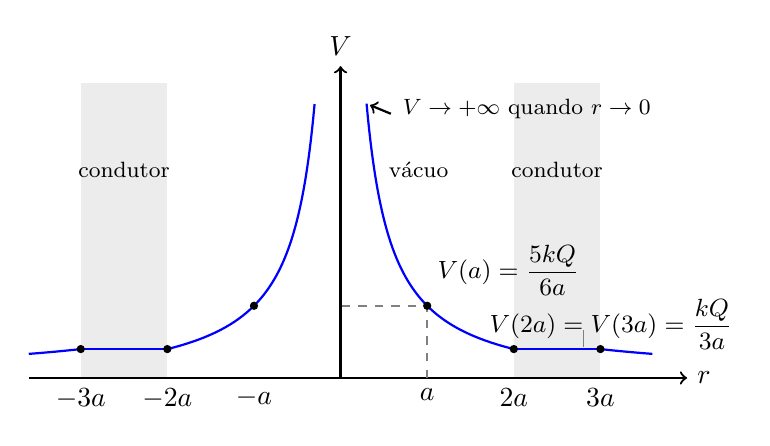
\begin{tikzpicture}[x=1.1cm,y=1.1cm,thick]
  \fill[gray!15] (2,0) rectangle (3,3.4);
  \fill[gray!15] (-3,0) rectangle (-2,3.4);
  \draw[->] (-3.6,0) -- (4.0,0) node[right] {$r$};
  \draw[->] (0,0) -- (0,3.6) node[above] {$V$};
  \draw[blue,domain=0.3:2,samples=120] plot (\x,{1/\x-1/6});
  \draw[blue,domain=-2:-0.3,samples=120] plot (\x,{-1/\x-1/6});
  \draw[blue,domain=3:3.6,samples=40] plot (\x,{1/\x});
  \draw[blue,domain=-3.6:-3,samples=40] plot (\x,{-1/\x});
  \draw[blue] (2,{1/3}) -- (3,{1/3});
  \draw[blue] (-3,{1/3}) -- (-2,{1/3});
  \draw[dashed,gray] (1,0) -- (1,{5/6}) -- (0,{5/6});
  \fill (1,{5/6}) circle (1.5pt);
  \fill (-1,{5/6}) circle (1.5pt);
  \fill (2,{1/3}) circle (1.5pt);
  \fill (-2,{1/3}) circle (1.5pt);
  \fill (3,{1/3}) circle (1.5pt);
  \fill (-3,{1/3}) circle (1.5pt);
  \node[below] at (1,0) {$a$};
  \node[below] at (-1,0) {$-a$};
  \node[below] at (2,0) {$2a$};
  \node[below] at (-2,0) {$-2a$};
  \node[below] at (3,0) {$3a$};
  \node[below] at (-3,0) {$-3a$};
  \node[above right] at (1,{5/6}) {\small $V(a)=\dfrac{5kQ}{6a}$};
  \draw[gray,thin] (2.8,0.36) -- (2.8,0.55);
  \node[anchor=west] at (1.6,0.62) {\small $V(2a)=V(3a)=\dfrac{kQ}{3a}$};
  \node at (0.9,2.4) {\footnotesize vácuo};
  \node at (2.5,2.4) {\footnotesize condutor};
  \node at (-2.5,2.4) {\footnotesize condutor};
  \node[anchor=west] at (0.6,3.1) {\footnotesize $V\to+\infty$ quando $r\to 0$};
  \draw[->] (0.58,3.05) -- (0.34,3.15);
\end{tikzpicture}
\end{center}
{\small Esboço: eixo horizontal em unidades de $a$ e vertical em unidades de $kQ/a$; escalas do desenho não são físicas. Faixas cinzas: condutor.}

\textbf{c)} Hipóteses adicionais.
\begin{itemize}
\item \emph{Fio ideal.} Ligadas pelo fio, as cascas formam um único condutor, com potencial comum $V$. Adota-se que o fio não retém carga ao ser retirado (capacitância desprezada). Isso é uma idealização explícita, não uma consequência de ``muito longo'': a capacitância de um fio cresce com o comprimento. Se o fio retivesse carga $q_f$, a soma das cargas das cascas seria $-q_f$, e o resultado dependeria de $q_f$, que o enunciado não fornece.
\item \emph{Influência mútua desprezível.} Como as cascas estão muito afastadas ($d\gg R_i$), $V_i=\dfrac{kq_i}{R_i}+\dfrac{kq_j}{d}\simeq\dfrac{kq_i}{R_i}$, em que $q_i$ é a carga líquida da casca $i$ (a carga central e a superfície interna se cancelam) e $R_1=2a$, $R_2=3a$.
\end{itemize}

\begin{enumerate}
\item \emph{Superfícies internas.} Gauss no metal de cada casca ($E=0$) envolve $+Q$ e a superfície interna. Logo cada superfície interna tem $-Q$, independentemente do fio.
\item \emph{Conservação.} As cascas começaram neutras e o sistema não troca carga com o exterior. Com $q_1$ (externa da casca 1, $r=2a$) e $q_2$ (externa da casca 2, $r=3a$):
\begin{align*}
(-Q+q_1)+(-Q+q_2)=0 \quad\Rightarrow\quad q_1+q_2=2Q.
\end{align*}
\item \emph{Potencial comum.} $V=\dfrac{kq_1}{2a}=\dfrac{kq_2}{3a}$, logo $q_2=\dfrac32\,q_1$.
\item \emph{Resolução.} $q_1+\dfrac32 q_1=2Q$ dá $q_1=\dfrac{4Q}{5}$, $q_2=\dfrac{6Q}{5}$ e $V=\dfrac{2kQ}{5a}$. Em forma geral, $q_i=\dfrac{2Q\,R_i}{R_1+R_2}$.
\end{enumerate}

Sentido: antes da ligação, $\dfrac{kQ}{2a}>\dfrac{kQ}{3a}$, logo passa carga positiva $Q/5$ da casca 1 para a casca 2 (equivalentemente, elétrons da casca 2 vão para a casca 1). Ao retirar o fio, que não retém carga, as cargas não mudam.

Verificações:
\begin{itemize}
\item Potenciais: $\dfrac{k\,(4Q/5)}{2a}=\dfrac{2kQ}{5a}=\dfrac{k\,(6Q/5)}{3a}$; cargas: $\left(-Q+\dfrac{4Q}{5}\right)+\left(-Q+\dfrac{6Q}{5}\right)=0$.
\item Energia (não circular): com as cargas internas fixas, $U=\dfrac{kq_1^2}{4a}+\dfrac{kq_2^2}{6a}+\text{const}$, com $q_1+q_2=2Q$. Antes, $U_{\rm i}=\dfrac{5kQ^2}{12a}$; depois, $U_{\rm f}=\dfrac{2kQ^2}{5a}$. A energia cai $\dfrac{kQ^2}{60a}$, dissipada no fio. Além disso, $\dfrac{\partial U}{\partial q_1}=V_1-V_2$ e $U$ é convexa em $q_1$; logo o mínimo com carga total fixa (teorema de Thomson) é onde $V_1=V_2$, ou seja, $q_1=\dfrac{4Q}{5}$.
\item Caso particular: se $R_1=R_2$, a fórmula dá $q_1=q_2=Q$, sem transferência, como esperado para potenciais iniciais iguais.
\end{itemize}

Resultados:
\begin{itemize}
\item Casca 1 (Figura 1): superfície interna ($r=a$) com $-Q$; superfície externa ($r=2a$) com $+\dfrac{4Q}{5}$; carga total $-\dfrac{Q}{5}$.
\item Casca 2 (Figura 2): superfície interna ($r=2a$) com $-Q$; superfície externa ($r=3a$) com $+\dfrac{6Q}{5}$; carga total $+\dfrac{Q}{5}$.
\end{itemize}

ANSWER: a) $V(a)=\dfrac{kQ}{2a}$; b) $V(a)=\dfrac{5kQ}{6a}$, $V(2a)=V(3a)=\dfrac{kQ}{3a}$, com gráfico contínuo, não crescente para $r\ge 0$, patamar entre $2a$ e $3a$ e divergência em $r\to 0$; c) casca 1: interna $-Q$ e externa $+\dfrac{4Q}{5}$; casca 2: interna $-Q$ e externa $+\dfrac{6Q}{5}$ (potencial comum final $\dfrac{2kQ}{5a}$).%
\newpage%
\section*{Questão 8}

\section*{Solução}

\textbf{Hipóteses e convenções.}
\begin{itemize}
\item (i) Sistema: a tonelada de suco, $m = 1000\ \text{kg}$, é um sistema fechado. Nas fases condensadas não há trabalho de eixo nem variação apreciável de volume, logo a energia trocada com o exterior é apenas calor. Convenção: $Q$ é o calor \emph{retirado} do suco, tomado como positivo.
\item (ii) Reservatórios: a câmara é a fonte fria, a $T_F = 246\ \text{K}$ ($-27\,^\circ$C), e o ambiente é a fonte quente, a $T_Q = 307{,}5\ \text{K}$ ($34{,}5\,^\circ$C), ambos com temperatura constante. Logo o COP do equipamento é constante, mesmo com o suco variando de temperatura. A câmara recebe todo o calor retirado do suco e o transfere ao evaporador, sem ganhos externos (hipótese revista na parte b).
\item (iii) Processo transitório: o suco esfria e muda de fase, mas o enunciado fornece apenas a duração total $\Delta t = 96\ \text{min} = 5760\ \text{s}$, sem perfil de carga. Com COP constante, o trabalho total é $W_{\text{total}} = Q/\text{COP}$, fixado pelos dados. A única potência constante que os dados determinam é a média $\overline{\dot W} = W_{\text{total}}/\Delta t$. Picos instantâneos podem ser maiores, mas não são calculáveis com os dados.
\item (iv) Calores específicos constantes em cada fase; solidificação isotérmica a $-2\,^\circ$C.
\item (v) Conversões: $1\ \text{kcal} = 1000\ \text{cal} = 4000\ \text{J}$; $1\ \text{HP} = 0{,}75\ \text{kW}$.
\end{itemize}

\textbf{a) Análise termodinâmica.}

\textit{Passo 1 (calor a retirar).} Balanço de energia no suco, que não recebe nem realiza trabalho: $-Q = \Delta U$. As trocas são de calor sensível (líquido e sólido) e de calor latente (solidificação, isotérmica). O calor total é a soma das três etapas, todas retiradas do suco:
\begin{align*}
Q_1 &= m\,c_L\,\bigl(33-(-2)\bigr) = 1000\cdot 1{,}0\cdot 35 = 35\,000\ \text{kcal}\\
Q_2 &= m\,L_f = 1000\cdot 72{,}5 = 72\,500\ \text{kcal}\\
Q_3 &= m\,c_S\,\bigl(-2-(-27)\bigr) = 1000\cdot 0{,}5\cdot 25 = 12\,500\ \text{kcal}
\end{align*}
Logo $Q = 120\,000\ \text{kcal}$ (120 kcal/kg). Com $1\ \text{kcal} = 4000\ \text{J}$,
\[
Q = 1{,}2\times10^{5}\cdot 4000\ \text{J} = 4{,}8\times10^{8}\ \text{J}.
\]

\textit{Passo 2 (taxa média de extração).} Pela hipótese (iii), e usando que o calor retirado da câmara é $Q$ por (ii),
\[
\dot Q_F = \frac{Q}{\Delta t} = \frac{4{,}8\times10^{8}}{5760}\ \text{W} = \frac{250\,000}{3}\ \text{W} \approx 83{,}3\ \text{kW}.
\]

\textit{Passo 3 (limite de Carnot).} Para um refrigerador reversível entre $T_F$ e $T_Q$, o COP é $\text{COP}_C = \dfrac{T_F}{T_Q-T_F}$, definido como $\dot Q_F/\dot W$. A bomba de calor, com $T_Q/(T_Q-T_F)$, não se aplica, porque o interesse é o calor retirado da câmara:
\[
\text{COP}_C = \frac{246}{307{,}5-246} = \frac{246}{61{,}5} = 4.
\]
Pelo teorema de Carnot (consequência da 2ª lei), nenhum refrigerador opera com COP maior que $\text{COP}_C$ entre as mesmas duas fontes.

\textit{Passo 4 (COP real).} Pelo enunciado,
\[
\text{COP} = \tfrac{3}{4}\,\text{COP}_C = \tfrac{3}{4}\cdot 4 = 3 < 4 = \text{COP}_C,
\]
o que é coerente com a 2ª lei. O fator $3/4$ já incorpora as irreversibilidades do ciclo.

\textit{Passo 5 (potência do compressor).} Por definição, $\text{COP} = \dot Q_F/\dot W$, em que $\dot W$ é a potência de acionamento do compressor:
\[
\dot W = \frac{\dot Q_F}{\text{COP}} = \frac{250\,000/3}{3}\ \text{W} = \frac{250\,000}{9}\ \text{W} \approx 27{,}8\ \text{kW}.
\]

\textit{Passo 6 (conversão).} Com $1\ \text{HP} = 0{,}75\ \text{kW}$,
\[
\dot W = \frac{27{,}8}{0{,}75}\ \text{HP} = \frac{1000}{27}\ \text{HP} \approx 37{,}0\ \text{HP}.
\]

\textit{Conferências.}
\begin{itemize}
\item 1ª lei no ciclo: $\dot Q_Q = \dot Q_F + \dot W = 83{,}3 + 27{,}8 = 111{,}1$ kW rejeitados ao ambiente, com $\dot Q_Q/\dot Q_F = 4/3 = (\text{COP}+1)/\text{COP}$. Todas as grandezas são positivas.
\item Energia por tonelada: $\dot W\,\Delta t = Q/\text{COP} = 1{,}6\times10^{8}$ J $\approx 44$ kWh.
\item Caso ideal: $\dot W_{\min} = \dot Q_F/4 \approx 20{,}8$ kW $\approx 27{,}8$ HP. A máquina real exige o fator $4/3$ sobre esse valor.
\item Sensibilidade: com $273{,}15$ K, $\text{COP}_C \approx 4{,}002$, variação de 0,06\%, desprezível.
\item Ordem de grandeza: $10^{8}$ J por tonelada e dezenas de kW de potência frigorífica, coerente com uma câmara industrial.
\end{itemize}

\textbf{b) Comparação com o engenheiro.}

Para 30 HP, $\dot W_{30} = 30\cdot 0{,}75 = 22{,}5$ kW. A capacidade de extração é
\[
\text{COP}\cdot\dot W_{30} = 3\cdot 22{,}5 = 67{,}5\ \text{kW} = 0{,}81\cdot 83{,}3\ \text{kW},
\]
ou seja, faltam cerca de 16 kW (19\%). O tempo de processo fica
\[
t = \frac{Q}{\text{COP}\cdot\dot W_{30}} = \frac{4{,}8\times10^{8}}{3\cdot 22\,500}\ \text{s} \approx 7{,}1\times10^{3}\ \text{s} \approx 118{,}5\ \text{min},
\]
cerca de 23\% acima dos 96 min previstos. Equivalentemente, cumprir 96 min com 30 HP exigiria COP $= Q/(\dot W_{30}\,\Delta t) \approx 3{,}70$, ou seja, 92,6\% do Carnot, contra os 75\% dados.

\textit{Sobre a folga.} Nem a máquina ideal de Carnot, que precisa de 27,8 HP, deixaria mais de 8\% de folga em 30 HP. A afirmação de folga não se sustenta.

\textit{Origem provável do 30 HP.} Os dados não confirmam nenhuma destas hipóteses, mas duas causas são plausíveis:
\begin{itemize}
\item Usar o COP de Carnot sem o fator $3/4$: $\dot W = 27{,}8$ HP, que arredondado daria 30 HP com folga de 8\%. Isso ignora um dado do enunciado.
\item Trocar o COP de refrigerador pelo de bomba de calor e aplicar o fator $3/4$: $\text{COP}_{BC} = \tfrac{3}{4}\cdot\tfrac{T_Q}{T_Q-T_F} = \tfrac{3}{4}\cdot 5 = 3{,}75$, logo $\dot W = 83{,}3/3{,}75 = 22{,}2$ kW $\approx 29{,}6$ HP $\approx 30$ HP. Esta é a confusão que mais reproduz o número 30 HP, mas está errada: o equipamento extrai calor da câmara, então seu desempenho é $\dot Q_F/\dot W$. Mesmo que o cálculo estivesse certo, a folga seria de apenas 1\%.
\end{itemize}

\textit{Completude: perdas reais.} O modelo é ideal. Perdas não incluídas no COP de 3/4 aumentariam a potência:
\begin{itemize}
\item ganho de calor por paredes, portas e embalagens entre o ambiente e a câmara ($\Delta T = 61{,}5$ K), que soma a $\dot Q_F$ e eleva $\dot W$ na mesma proporção;
\item partida (\emph{pull-down}) e degelo, que exigem potência acima da média;
\item rendimento do motor elétrico: a potência que aparece na conta de energia é $\dot W/\eta_m$, maior que a potência de eixo.
\end{itemize}
Logo, 37 HP é um piso (limite inferior), e não um valor de projeto.

\textbf{Conclusão.} A estimativa \textbf{não é procedente}. Os 30 HP extraem apenas cerca de 81\% da carga necessária, faltando cerca de 7 HP em relação a 37 HP, e o congelamento duraria cerca de 118,5 min, e não 96 min. Longe de haver folga, o compressor ficaria subdimensionado. Recomenda-se especificar no mínimo 37 HP de potência de eixo, com margem definida pelas perdas reais listadas acima.

ANSWER: a) $\dot W \approx 27{,}8$ kW $\approx 37$ HP (exato $1000/27$ HP), com $Q = 4{,}8\times10^{8}$ J extraídos em 96 min e COP real $= 3$; b) a estimativa de 30 HP não é procedente, pois esse compressor fornece apenas cerca de 81\% da potência necessária e congelaria a tonelada em cerca de 118,5 min, e não em 96 min.%
\newpage%
\section*{Questão 9}

\section*{Solução}

\textbf{Hipóteses.} Fontes pontuais, monocromáticas, de mesma frequência, coerentes (mesma fase inicial) e no mesmo meio homogêneo. Vale a superposição linear dos campos e $I=\mu A^2$, com $\mu$ constante e $A$ a amplitude do campo resultante. $I_1(\theta)$ é a intensidade que $F_1$ produziria sozinha em $P$, e $I_2=3I_1(\theta)$ em todo $P$, como dado. Como $L\gg a$, os raios de $F_1$ e $F_2$ até $P$ são quase paralelos; essa hipótese é usada na diferença de caminho. O ângulo $\theta$ é medido a partir da horizontal que passa pelo ponto médio $O$ entre as fontes.

\textbf{1) Razão das amplitudes.} Sejam $A_1,A_2>0$ as amplitudes de cada fonte em $P$. Como $I_j=\mu A_j^2$ e $I_2=3I_1$,
\[
A_2=\sqrt{3}\,A_1 .
\]

\textbf{2) Diferença de caminho.} Tome $O=(0,0)$, o anteparo em $x=L$, $F_1=(0,a/2)$, $F_2=(0,-a/2)$ e $P=(L,y)$, com $y=L\tan\theta$ e $R=OP=L/\cos\theta$. Usando $L^2+y^2=R^2$ e $y=R\sin\theta$, com $r_j=F_jP$,
\[
r_1^2=L^2+\left(y-\tfrac a2\right)^2=R^2-aR\sin\theta+\tfrac{a^2}{4},\qquad
r_2^2=R^2+aR\sin\theta+\tfrac{a^2}{4}.
\]
Assim $r_2^2-r_1^2=2aR\sin\theta$ e
\[
\Delta r=r_2-r_1=\frac{2aR\sin\theta}{r_1+r_2}.
\]
Como $a/R\le a/L\ll 1$ para todo $\theta$, expande-se $\sqrt{R^2+u}\approx R+\tfrac{u}{2R}$, com erro $O(a^2/R)$:
\[
r_{1,2}=R\mp\tfrac a2\sin\theta+O\!\left(\tfrac{a^2}{L}\right)
\quad\Rightarrow\quad
r_1+r_2=2R\left[1+O\!\left(\tfrac{a^2}{L^2}\right)\right].
\]
Logo
\[
\Delta r=a\sin\theta\left[1+O\!\left(\tfrac{a^2}{L^2}\right)\right]\simeq a\sin\theta .
\]
Geometricamente, $\Delta r$ é a projeção de $\overrightarrow{F_2F_1}$ (vertical, módulo $a$) sobre a direção de $OP$. Como as fontes estão em fase, a diferença de fase em $P$ vem só do caminho:
\[
\varphi=k\,\Delta r\simeq q\sin\theta,\qquad k=\frac{2\pi}{\lambda},\quad q=\frac{2\pi a}{\lambda}.
\]

\textbf{3) Resultante (item a).} Tomando a fase de $F_1$ como referência, o campo em $P$ é
\[
E=A_1\cos\omega t+A_2\cos(\omega t-\varphi)=\mathrm{Re}\left\{\left(A_1+A_2e^{-i\varphi}\right)e^{i\omega t}\right\}.
\]
Sua amplitude é $|A_1+A_2e^{-i\varphi}|$. Pela observação do enunciado ($I\propto A^2$),
\[
I=\mu\left|A_1+A_2e^{-i\varphi}\right|^2=I_1+I_2+2\sqrt{I_1I_2}\cos\varphi .
\]
Com $I_2=3I_1$ e $\sqrt{I_1I_2}=\sqrt{3}\,I_1$:
\[
I(\theta)=I_1(\theta)\left[4+2\sqrt{3}\,\cos\!\left(\frac{2\pi a\sin\theta}{\lambda}\right)\right].
\]
Conferências: a média de $I$ sobre um período de $\varphi$ é $I_1+I_2=4I_1$, pois o termo cruzado tem média nula sobre um período. Para $I_2=\beta I_1$ genérico, $I=I_1(1+\beta+2\sqrt{\beta}\cos\varphi)$; com $\beta=1$ recai em $4I_1\cos^2(\varphi/2)$, o resultado clássico.

\textbf{4) Extremos do fator de franja.} Escreva $I=I_1(\theta)\,g(\theta)$, com $g=4+2\sqrt{3}\cos\varphi$. Para $0<\theta<\pi/2$, $\varphi=q\sin\theta$ cresce monotonicamente de $0$ a $q$, e
\[
\frac{dg}{d\theta}=-2\sqrt{3}\,q\cos\theta\,\sin\varphi=0\iff\varphi=n\pi\iff a\sin\theta=\frac{n\lambda}{2},\qquad n=1,2,\dots
\]
Para $n$ par, $g=4+2\sqrt{3}=(1+\sqrt{3})^2$ é máximo; para $n$ ímpar, $g=4-2\sqrt{3}=(\sqrt{3}-1)^2$ é mínimo.

Efeito de $I_1$: $I'=I_1\left(g'+L_1g\right)$, com $L_1=d\ln I_1/d\theta$. Resolvendo $I'=0$ perto de $\varphi=n\pi$, os extremos se deslocam de $\delta\theta=O\!\left(|L_1|\lambda^2/a^2\right)$ rad. Assim, para $a\gg\lambda$ e $I_1$ de variação suave na escala da franja, as posições são as de $g$; se $I_1$ é constante, são exatas.

\textbf{5) Primeiro máximo com $\theta>0$ (item b).} Pelo passo 4, os extremos com $\theta>0$ aparecem na ordem $n=1,2,\dots$. O caso $n=0$ é o máximo central em $\theta=0$, excluído pelo enunciado. O primeiro extremo ($n=1$) é mínimo, logo o primeiro máximo é $n=2$, isto é, $a\sin\theta_1=\lambda$:
\[
\sin\theta_1=\frac{\lambda}{a},\qquad
I_{\max}=(4+2\sqrt{3})\,I_1(\theta_1)=(1+\sqrt{3})^2\,I_1(\theta_1)\approx 7{,}46\,I_1(\theta_1).
\]
Condição de existência: $\sin\theta_1<1$, ou seja, $a>\lambda$. Para $a\le\lambda$, $\varphi<2\pi$ em todo $0<\theta<\pi/2$ e não há máximo de interferência nesse intervalo. A forma $(1+\sqrt{3})^2=(A_1+A_2)^2/A_1^2$ corresponde à soma em fase.

\textbf{6) Primeiro mínimo com $\theta>0$ (item c).} É o extremo $n=1$, isto é, $a\sin\theta_2=\lambda/2$:
\[
\sin\theta_2=\frac{\lambda}{2a},\qquad
I_{\min}=(4-2\sqrt{3})\,I_1(\theta_2)=(\sqrt{3}-1)^2\,I_1(\theta_2)\approx 0{,}536\,I_1(\theta_2).
\]
Condição de existência: $\sin\theta_2<1$, ou seja, $a>\lambda/2$. O mínimo não se anula porque $A_1\neq A_2$; a anulação exigiria $I_1=I_2$, o que contradiz $I_2=3I_1$. A forma $(\sqrt{3}-1)^2=(A_2-A_1)^2/A_1^2$ corresponde à subtração das ondas em oposição de fase.

\textbf{Conferências.}
\begin{itemize}
\item Razão: para o fator de franja, $g_{\max}/g_{\min}=(2+\sqrt{3})^2\approx 13{,}9$. Com $I_1$ dependente de $\theta$, a razão das intensidades é $I_{\max}/I_{\min}=(2+\sqrt{3})^2\,I_1(\theta_1)/I_1(\theta_2)$; para $I_1=\cos^2\theta$ e $a=5\lambda$, isso dá $\approx 13{,}5$. Além disso, $I_{\max}>\langle I\rangle=4I_1>I_{\min}$.
\item Numérico ($I_1=\cos^2\theta$, $a=5\lambda$, $L=10^{6}\lambda$, diferença de caminho exata): o máximo exato está em $0{,}20043$ rad, contra $0{,}20136$ rad previsto ($\theta_1=\arcsin 0{,}2$). O valor de $I$ nesse ponto difere de $(4+2\sqrt{3})I_1(\theta_1)$ em $0{,}019\%$.
\item Unidades e ordens de grandeza: $\lambda$ e $a$ na mesma unidade; $\sin\theta$ e o argumento do cosseno são adimensionais. Para $a=5\lambda$: $\theta_1\approx 11{,}5^\circ$ e $\theta_2\approx 5{,}7^\circ$. Os ângulos são pequenos porque $a\gg\lambda$, e não por $L\gg a$.
\item Validade: (b) exige $a>\lambda$ e (c) exige $a>\lambda/2$. Para $a$ não muito maior que $\lambda$, a variação de $I_1$ pode criar extremos de $I$ que não são de interferência. Por exemplo, com $I_1=\cos^2\theta$ e $a=0{,}8\lambda$, há um máximo local de $I$ perto de $1{,}02$ rad, sem máximo de interferência. Os itens (b) e (c) referem-se aos extremos de interferência.
\end{itemize}

ANSWER: a) $I(\theta)=I_1(\theta)\left[4+2\sqrt{3}\cos\left(\frac{2\pi a\sin\theta}{\lambda}\right)\right]$; b) $I_{\max}=(4+2\sqrt{3})\,I_1(\theta_1)\approx 7{,}46\,I_1(\theta_1)$, com $\sin\theta_1=\lambda/a$ (para $a>\lambda$); c) $I_{\min}=(4-2\sqrt{3})\,I_1(\theta_2)\approx 0{,}536\,I_1(\theta_2)$, com $\sin\theta_2=\lambda/(2a)$ (para $a>\lambda/2$).%
\newpage%
\section*{Questão 10}

\section*{Solução}

\textbf{Hipóteses e notação.} Óptica geométrica (feixe estreito), meio homogêneo, espelhos ideais com reflexão especular. O feixe está num plano perpendicular ao eixo, logo o problema é bidimensional: tomamos o centro $O$ sobre o eixo e coordenadas polares $(\rho,\varphi)$. Entre reflexões consecutivas o feixe é retilíneo e permanece em $r<\rho<R$. Seja $\alpha$ o ângulo de incidência em $A$ (espelho externo), medido em relação à normal $OA$, e $\theta$ o ângulo de incidência em $B$ (espelho interno), medido entre o feixe e o prolongamento radial de $OB$, como na figura. Pela lei da reflexão, a normal em cada ponto de reflexão é a radial e o raio refletido é simétrico do incidente em relação a ela.

\textbf{Passo 1 -- Ângulo central.} No triângulo $OAB$ temos $\angle OAB=\alpha$ e $\angle OBA=\pi-\theta$ (suplementar de $\theta$). Sendo $\Delta\varphi=\angle AOB$, a soma dos ângulos internos dá
\[
\Delta\varphi=\pi-\alpha-(\pi-\theta)=\theta-\alpha .
\]

\textbf{Passo 2 -- Lei dos senos.} Em $OAB$: $\dfrac{OA}{\sin\angle OBA}=\dfrac{OB}{\sin\angle OAB}$, isto é, $\dfrac{R}{\sin\theta}=\dfrac{r}{\sin\alpha}$. Logo
\[
\sin\alpha=\frac{r}{R}\,\sin\theta=\frac{\sqrt{3}}{2}\,\sin\theta . \tag{1}
\]

\textbf{Passo 3 -- Intervalos dos ângulos.} Seja $X(t)=B+t\,\vec u$, com $\vec u=A-B$ e $0\le t\le 1$. Então
\[
|X|^2=r^2+2t\,\vec B\cdot\vec u+t^2|\vec u|^2 .
\]
Para que $X$ permaneça em $\rho\ge r$ logo após $B$, é preciso $\vec B\cdot\vec u\ge 0$, isto é, $\cos\theta\ge 0$, pois $\vec B\cdot\vec u=r\,|\vec u|\cos\theta$. Analogamente, junto a $A$ deve valer $\rho\le R$, o que exige $\cos\alpha\ge 0$. Se $\theta=0$, (1) dá $\alpha=0$ e $\Delta\varphi=0$: o feixe é radial, não há avanço angular, caso degenerado excluído. O caso $\theta=\pi/2$ (rasância) é tratado no item b. Assim
\[
0<\theta<\frac{\pi}{2},\qquad 0<\alpha<\frac{\pi}{2}.
\]
Como $\sin\alpha<\sin\theta$ e o seno é crescente em $(0,\pi/2)$, vale $\alpha<\theta$, o que confirma $\Delta\varphi>0$.

\textbf{Passo 4 -- Reflexões sucessivas.} Sejam $P_0=A$, $P_1=B$, $P_2,P_3,\dots$ os pontos de reflexão seguintes e $S_k$ a reflexão do plano na reta $OP_k$. Pela lei da reflexão, a direção de saída em $P_k$ é a simétrica, em relação à normal $OP_k$, da direção $P_k\to P_{k-1}$. Como $S_k$ fixa $O$ e $P_k$, o ponto $S_k(P_{k-1})$ está sobre o raio de saída, e
\[
P_{k+1}=S_k(P_{k-1}).
\]
Sendo $S_k$ uma isometria que fixa $O$, o segmento $P_kP_{k+1}$ é imagem de $P_kP_{k-1}$: tem o mesmo comprimento, o mesmo $\Delta\varphi$ e interior em $r<\rho<R$. Em polares, $S_k$ leva $\varphi\mapsto 2\varphi_k-\varphi$ e preserva $\rho$, donde $\varphi_{k+1}-\varphi_k=\varphi_k-\varphi_{k-1}$ e $\rho_{k+1}=\rho_{k-1}$. Com $\varphi_0=0$ e $\varphi_1=\Delta\varphi>0$, por indução
\[
\varphi_k=k\,\Delta\varphi ,
\]
e os raios alternam $R,r,R,\dots$ (espelho externo para $k$ par, interno para $k$ ímpar). Como todos os avanços são iguais e positivos, o feixe gira sempre no mesmo sentido e os avanços não se cancelam.

\textbf{Passo 5 -- Fechamento após uma volta.} O estado do feixe em $P_k$ é determinado pelo par $(P_{k-1},P_k)$. Dizer que os raios se sobrepõem após uma volta significa que, ao completar o avanço angular $2\pi$, o feixe volta a $A$ com a mesma direção, isto é, $P_N=A$ e $P_{N+1}=B$, sendo $N$ o número de reflexões nessa volta. Então:
\begin{itemize}
\item $N\,\Delta\varphi=2\pi$, pois o avanço angular numa volta é $2\pi$;
\item $P_N=A$ está no espelho externo; como $\rho_k=R$ somente para $k$ par, $N$ é par;
\item há $n$ pontos de reflexão em cada espelho por volta; os externos são $P_0,P_2,\dots,P_{2n-2}$ (ângulos $2j\pi/n$, distintos) e os internos são $P_1,P_3,\dots,P_{2n-1}$. Logo $N=2n$, e a sobreposição ocorre já nessa primeira volta.
\end{itemize}
Portanto $2n\,\Delta\varphi=2\pi$, isto é,
\[
\theta-\alpha=\Delta\varphi=\frac{\pi}{n}. \tag{2}
\]

\textbf{Passo 6 -- Equação para $\theta$.} Substituindo $\alpha=\theta-\pi/n$ em (1):
\[
\sin\Big(\theta-\frac{\pi}{n}\Big)=\frac{\sqrt3}{2}\sin\theta
\;\Longrightarrow\;
\sin\theta\Big(\cos\frac{\pi}{n}-\frac{\sqrt3}{2}\Big)=\cos\theta\,\sin\frac{\pi}{n}. \tag{3}
\]
Como $\cos\theta>0$ (Passo 3), dividimos por $\cos\theta$ e obtemos
\[
\tan\theta\Big(\cos\frac{\pi}{n}-\frac{\sqrt3}{2}\Big)=\sin\frac{\pi}{n}. \tag{4}
\]
(Se $\cos\theta=0$, (3) só vale com $n=6$, caso tratado no item b.)

\textbf{a)} Como $\sqrt3/2=\cos(\pi/6)$, o denominador é $\cos(\pi/n)-\cos(\pi/6)$, que se anula apenas para $n=6$. Logo, para $n\neq 6$,
\[
\tan\theta=\frac{\sin(\pi/n)}{\cos(\pi/n)-\sqrt3/2}=\frac{2\sin(\pi/n)}{2\cos(\pi/n)-\sqrt3}.
\]

\textbf{b) Valores possíveis de $n$.}
\begin{itemize}
\item $n\le 2$: por (2) e $\alpha>0$, $\pi/n=\theta-\alpha<\theta<\pi/2$, logo $n\ge 3$. Isso exclui $n=1$ e $n=2$.
\item $3\le n\le 5$: $\pi/n>\pi/6$, logo $\cos(\pi/n)<\sqrt3/2$. Com $\sin(\pi/n)>0$, o lado direito de (a) é negativo, mas $\tan\theta>0$ em $(0,\pi/2)$. Impossível.
\item $n=6$: o denominador se anula e (3) dá $\tfrac12\cos\theta=0$, logo $\theta=\pi/2$. Geometria: $AB=\sqrt{R^2-r^2}=R/2$ e $\cos\angle AOB=r/R$, logo $\angle AOB=\pi/6$. O feixe apenas tangencia o cilindro interno em $B$ (rasância): a direção não muda e não há reflexão efetiva em $B$. A órbita degenera no hexágono regular inscrito no círculo de raio $R$ (cada corda $AA'=2AB=R$ subtende $60^\circ$ e seu ponto médio está à distância $R\cos 30^\circ=r$ de $O$), com reflexões só no espelho externo. Excluído.
\item $n\ge 7$: $\cos(\pi/n)>\sqrt3/2$, o denominador é positivo e $\tan\theta=T_n>0$, logo $\theta=\arctan T_n\in(0,\pi/2)$. Como $0<\cos(\pi/n)-\sqrt3/2<\cos(\pi/n)$ e $\sin(\pi/n)>0$, tem-se $T_n>\tan(\pi/n)$, donde $\theta>\pi/n$ e $\alpha=\theta-\pi/n\in(0,\theta)$.

\emph{Existência.} Tome um triângulo com $OA=R$, $OB=r$ e $\angle AOB=\pi/n$. Sejam $\alpha^*=\angle OAB$ e $\theta^*=\pi-\angle OBA\in(0,\pi)$. A soma dos ângulos dá $\alpha^*=\theta^*-\pi/n$, e a lei dos senos dá $\sin\alpha^*=\frac{\sqrt3}{2}\sin\theta^*$, que é (3). Se $\cos\theta^*=0$, (3) daria $\sin\theta^*\big(\cos\frac{\pi}{n}-\frac{\sqrt3}{2}\big)=0$, impossível para $n\ge 7$. Logo vale (4), com $\tan\theta^*=T_n>0$; como $\theta^*\in(0,\pi)$, resulta $\theta^*=\theta$. Assim $\cos\theta>0$, e ao longo de $AB$ tem-se $\frac{d}{dt}|X|^2=2r|\vec u|\cos\theta+2t|\vec u|^2>0$: $\rho$ cresce estritamente de $r$ em $B$ até $R$ em $A$, sem tocar os cilindros no interior do segmento. Portanto $B$ é o primeiro contato, e os Passos 4 e 5 garantem o fechamento após $2n$ reflexões.
\end{itemize}
Conclusão: $n\ge 7$, sem limite superior.

\textbf{Conferências.} Ângulos, $r/R$ e $\tan\theta$ são adimensionais, e (4) é homogênea em ângulos. O sinal é coerente: $\tan\theta>0$ exige $\cos(\pi/n)>\sqrt3/2$, isto é, $n\ge 7$, como concluído em b.
\begin{itemize}
\item $n=7$: $\sin(\pi/7)\approx 0{,}4339$ e $\cos(\pi/7)-\sqrt3/2\approx 0{,}0349$, logo $\tan\theta\approx 12{,}42$, $\theta\approx 85{,}40^\circ$ e $\alpha=\theta-\pi/7\approx 59{,}68^\circ$. Teste em (1): $\sin\alpha\approx 0{,}8632$ e $\frac{\sqrt3}{2}\sin\theta\approx 0{,}8660\cdot 0{,}99677\approx 0{,}8632$, em concordância.
\item $n=8$: $\tan\theta\approx 6{,}61$ e $\theta\approx 81{,}40^\circ$.
\item Limite $n\to\infty$: $\tan\theta\approx\dfrac{\pi/n}{1-\sqrt3/2}=(4+2\sqrt3)\dfrac{\pi}{n}\to 0$. O feixe torna-se quase radial, com $\theta$, $\alpha$ e $\Delta\varphi$ tendendo a zero, coerente com o Passo 3.
\end{itemize}

ANSWER: a) $\tan\theta=\dfrac{\sin(\pi/n)}{\cos(\pi/n)-\sqrt{3}/2}=\dfrac{2\sin(\pi/n)}{2\cos(\pi/n)-\sqrt{3}}$ (para $n\neq 6$); b) $n\geq 7$, isto é, $n\in\{7,8,9,\dots\}$%
\newpage%
\section*{Apêndice: parecer do avaliador}%
\subsection*{Questão 1: nota 8,5 (não aprovada, rodada 3 de 3)}%
\textbf{Resposta da resolução às cegas do avaliador:} a) Movimento oscilatório com posições possíveis -2 < x < 4 (em metros). Para uma energia E $\in$ (0, 32/3), o movimento vai de x$_{1}$ $\in$ (-2, 0) até x$_{2}$ $\in$ (0, 4), raízes de (x - 4)$^2$(x + 2) = 32 - 3E. A condição vem de E\_p(x) - 32/3 = -(1/3)(x - 4)$^2$(x + 2), e E\_p(-2) = E\_p(4) = 32/3.\newline%
\newline%
b) E\_sup = 32/3 J $\approx$ 10,67 J (supremo não atingido; a altura da barreira em x = 4 é E\_p(4) = 32/3).\newline%
\newline%
c) Gráfico v(t) não periódico. Começa em -v$_{0}$ com tangente horizontal em t = 0. Sobe até 0 no retorno em x\_L < -2. Chega a +v$_{0}$ em x = 0 com tangente horizontal. Decresce até o mínimo v$_{4}$ = $\surd$(2(E - 32/3)/m) > 0 em x = 4, com tangente horizontal. Depois cresce sem limite, com v $\to$ +$\infty$ em tempo finito t*.\par %
Resposta final correta e igual à referência nos três itens. (a) -2 m < x < 4 m, com 0 < E < 32/3 J. (b) E\_sup = 32/3 J $\approx$ 10,67 J, supremo não atingido. (c) v(0) = -$\surd$(2E/m); a velocidade se anula em x\_t < -2, volta a +v$_{0}$ em x = 0, tem mínimo local v$_{4}$ > 0 em x = 4 e diverge para +$\infty$ em tempo finito, sem oscilação.\newline%
\newline%
Verificações feitas em Python puro (numpy não está disponível): a identidade E\_p = 32/3 - (x-4)$^2$(x+2)/3 = x$^2$(6-x)/3 e F = -dE\_p/dx conferem; E\_p(-2) = E\_p(4) = 32/3 e E\_p'(-2) = -12; a fatoração E - E\_p = (x-x\_L)(x$_{2}$-x)(x$_{3}$-x)/3 é exata; o semiperíodo perto de E\_sup dá t\_\{L$\to$2\} - ¼ ln(1/$\delta$) $\to$ 2,1089, o que confirma o 2,109 citado; no exemplo E = 16 J, m = 1, a integração RK4 e a quadratura dão t$_{1}$ = 0,640, t$_{2}$ = 1,280 (= 2t$_{1}$), t$_{3}$ = 2,192, v$_{4}$ = 3,266, v(3 s) = 12,60, v(3,25 s) = 31,08 e t* $\approx$ 3,975, todos batendo com o texto.\newline%
\newline%
Todas as armadilhas listadas foram tratadas: união das oscilações em (a), componente conexa e ilimitada, x = -2 não é extremo, condição E > 0, x > 6 não é poço, supremo e não máximo em (b), v(0) < 0, não periodicidade, tangente horizontal em t = 0, t$_{3}$ e t$_{2}$, divergência em tempo finito, massa simbólica, sinal de F e unidades. Não há erro de conteúdo nem critical ou major. A nota fica em 8,5 pelas lacunas de rigor: a não{-}periodicidade de (b) para E > 32/3 é argumentada só para um caso, o termo O(1) do período extra é hand{-}waved, e a frase sobre retornos em (b) para E = 32/3 é contraditória.%
\begin{itemize}%
\item%
{[}minor{]} Item (b), E > 32/3: a não{-}periodicidade é justificada só para trajetórias que chegam a x $\geq$ 0 com v > 0 ("uma vez em x$\geq$0 com v>0, não pode voltar"). O argumento completo é que \{E\_p $\leq$ E\} = {[}x\_t, $\infty$), com um único ponto de retorno, logo não há região limitada e não há movimento periódico, qualquer que seja a condição inicial. Deve ser escrito explicitamente.%
\item%
{[}minor{]} Item (b), E = 32/3: a frase "Em nenhum caso há retorno a um ponto de retorno após excursão finita" contradiz o caso (i), em que a partícula reflete em x = -2 após excursão finita. Deve ser trocada por algo como "não há segundo retorno / a trajetória não é periódica".%
\item%
{[}minor{]} Trecho extra "Período perto de E\_sup", não pedido. O resultado está correto: verifiquei que t\_\{L$\to$2\} - ¼ ln(1/$\delta$) $\to$ 2,1089 para $\delta$ = 10$^{-}$$^2$, 10$^{-}$$^3$, 10$^{-}$$^{4}$, e o valor 2,109 do texto confere. Porém o termo O(1) é justificado só com "fator 1+O(u)" e "quantidade limitada". Faltam a mudança de variável w = u$\surd$(1-u/6), ou um limite para a integral da diferença. A citação da "simetria temporal do item (c)" também sugere que o argumento é específico de E > 32/3, quando vale para qualquer ponto de retorno simples.%
\item%
{[}minor{]} Item (a), caso x$_{0}$ > 4: tratado em uma única frase ("proibida ou pertence a componente ilimitada"). Deveria afirmar que, para 0 < E < 32/3, a região de x > 4 é {[}x$_{3}$(E), $\infty$), ilimitada e separada do poço pela barreira, e que para E $\leq$ 0 ou E $\geq$ 32/3 não há poço nessa região.%
\item%
{[}minor{]} Notação: x\_L (no item a) e x\_t (nos itens b e c) designam o mesmo ponto de retorno esquerdo, em faixas de energia diferentes. Isso pode confundir o leitor. Convém unificar a notação ou avisar explicitamente.%
\item%
{[}minor{]} Exemplo numérico do item (c) com m = 1 kg e E = 16 J, que não está no enunciado. Está rotulado como exemplo e os valores conferem (t$_{1}$ $\approx$ 0,640; t$_{2}$ $\approx$ 1,280; t$_{3}$ $\approx$ 2,192; v$_{4}$ $\approx$ 3,266; v(3 s) $\approx$ 12,60; x\_t $\approx$ -2,392; t* $\approx$ 3,975). Mas o texto não descreve o método numérico e não diz que os tempos escalam com $\surd$m e as velocidades com 1/$\surd$m.%
\end{itemize}%
\subsection*{Questão 2: nota 9,0 (aprovada, rodada 1 de 1)}%
\textbf{Resposta da resolução às cegas do avaliador:} a) R\_A/R\_B = 16/9 ($\approx$ 1,78). Kepler: (R\_A/R\_B)$^3$ = (T\_A/T\_B)$^2$, com T\_A = 640 e T\_B = 270 dias terrestres.\newline%
b) v\_A/v\_B = 3/4 (v = 2$\pi$R/T, ou v $\propto$ R\^{}(-1/2)).\newline%
c) M\_B/M\_CA = 1/8 (ou seja, M\_CA = 8 M\_B). Razão das gravidades superficiais, com $\rho$ e M\_S cancelando: (8,1$\times$10$^{-}$$^{4}$/2,048$\times$10$^{-}$$^2$)$\cdot$(16/9)$^2$ = 1/8.\newline%
d) v\_B/v\_CA = 2 (v\_CA = v\_B/2). Obtido pela energia mecânica após o choque, E\_CA = 7E\_B, em r = R\_A.\newline%
e) Apoastro. Em R\_A, v\_CA$^2$ = (4/9)$\cdot$v\_circ(R\_A)$^2$ < v\_circ$^2$, e a órbita tem a = 8R\_B/7 < R\_A. O ponto de colisão é o mais afastado de S (periastro em r $\approx$ 0,51 R\_B, e = 5/9).\par %
Todas as cinco respostas coincidem com a referência e foram conferidas: (a) R\_A/R\_B = 16/9; (b) v\_A/v\_B = 3/4; (c) M\_B/M\_CA = 1/8; (d) v\_B/v\_CA = 2; (e) apoastro. Reli o enunciado no PDF e a transcrição confere. Refiz as contas com frações exatas no Python. A resolução trata as armadilhas: conversão de unidades (640 e 270 dias terrestres), Kepler com expoente correto, v = 2$\pi$r/T, cancelamento de R pela igualdade de dimensões, percentuais como 8,1$\times$10$^{-}$$^{4}$ e 2,048$\times$10$^{-}$$^2$, E\_CA = +7E\_B com ambas negativas, potencial avaliado em r\_A, inversão correta em (d). No item (e), o argumento é completo: o ponto é ápside, v\_CA = (2/3) v\_circ(r\_A), a = 9r\_A/14 < r\_A e e = 5/9. Não há erro de conta nem salto lógico. Os problemas restantes são de hipóteses não declaradas e de justificativas breves. Nota 9: publicável como gabarito comentado após pequenos ajustes."%
\begin{itemize}%
\item%
{[}minor{]} A hipótese de planetas esféricos não é declarada. A razão de gravidades do item (c) usa GM/R$^2$ na superfície, o que pressupõe simetria esférica. Deveria constar nas hipóteses iniciais, como faz a referência.%
\item%
{[}minor{]} As duas observações do enunciado sobre o cometa C (efeito gravitacional nas órbitas antes do choque) e sobre a interação A--B não são citadas. A resolução só as usa implicitamente, ao supor órbitas circulares não perturbadas antes do choque em (d) e (e). Deveria citá{-}las nas hipóteses.%
\item%
{[}minor{]} A hipótese (iv), de que o impulso da gravidade de S durante o choque é desprezível, é afirmada sem justificativa. A tangencialidade de v\_CA depende dela. Deveria dizer explicitamente que a duração do choque é pequena frente ao período orbital.%
\item%
{[}minor{]} No item (d), não se explica por que o momento linear não basta (massa e velocidade de C são desconhecidas) e por que a energia pós{-}choque fecha o problema. Uma frase bastaria. A dispensa de separar M\_A e M\_C está correta, mas o motivo não é dito.%
\item%
{[}minor{]} Terminologia: 'apsis' (usado em (v) e (e)) não é o termo em português. Deveria ser 'ápside' ou 'apsíde'. Trata{-}se de detalhe de linguagem.%
\item%
{[}minor{]} Opcional, para reforçar o item (e): a conferência não verifica o periastro. Faltaria mostrar que r\_p = 2r\_A/7 = 32R\_B/63 satisfaz a energia (v\_p = 1,75 v\_B; E/M = -0,4375 v\_B$^2$) ou conservação do momento angular na outra extremidade.%
\end{itemize}%
\subsection*{Questão 3: nota 8,5 (não aprovada, rodada 2 de 3)}%
\textbf{Resposta da resolução às cegas do avaliador:} (a) d\_min = 3?/5. A trajetória após B é uma semicircunferência de centro B e raio ? - d. A tração é mínima no topo, T\_topo = mg{[}2d/(? - d) - 3{]}. Exigir T\_topo $\geq$ 0 dá 5d $\geq$ 3?. Isso vale para 3?/5 $\leq$ d < ?. No limite d = 3?/5 a tração no topo é zero.\newline%
\newline%
(b) R = ?/14 ($\approx$ 0,071?). Com d = 3?/7 < 3?/5 o fio folga antes do topo, em $\varphi$* com cos $\varphi$* = 1/2 (60$^\circ$ a partir da vertical de B, ou 30$^\circ$ acima da horizontal de B). A esfera então segue uma parábola, com velocidade v*$^2$ = 2g?/7 a 60$^\circ$ da horizontal. No apogeu, que é o ponto mais alto após B (11?/28 acima de B), v?$^2$ = g?/14 e R = v?$^2$/g = ?/14.\newline%
\newline%
Não há alternativas de múltipla escolha nesta questão.\par %
Ambas as respostas finais conferem com a referência: (a) d\_min = 3?/5 e (b) raio de curvatura ?/14. Verifiquei o enunciado no PDF (página 3), que confere com a transcrição. Refiz a dedução e rodei uma simulação RK4 da dinâmica completa (sim\_q3.py, na pasta judge): fio tracionado até o topo para d $\geq$ 0,600? e folga para d = 0,599?; para d = 3?/7 o fio folga em sin$\theta$ = 1/2 (ponto (-2$\surd$3?/7, 2?/7) relativo a B), engata de novo em (0,-R) relativo a B, e o apogeu fica em 11?/28 acima de B com raio 0,071429? = ?/14. O candidato acertou tudo que a referência e as armadilhas exigem: queda ? com v$_{0}$$^2$ = 2g?, raio ?-d após o engate sem perda no engate, T $\geq$ 0 em todo o arco com o topo como ponto crítico, limiar 3?/5 $\leq$ d < ?, folga antes do topo, velocidade a 60$^\circ$ da horizontal, apogeu como ponto mais alto (inclusive após o engate, onde o pêndulo fica em -27?/28 relativo a A), e R = v?$^2$/g. As verificações de folga e de não contato com a barra são explícitas e corretas. Os problemas são de rigor e apresentação, nenhum altera o resultado: hipótese do impulso inelástico não declarada, ressalva da barra tratada só como observação, notação e referencial alternados, e algumas equações escritas sem a justificativa completa. Nota 8,5: quase gabarito comentado; faltam o fechamento das hipóteses e uma notação única para publicar."%
\begin{itemize}%
\item%
{[}minor{]} O engate do fio em (0,-R) é tratado como impulso radial perfeitamente inelástico, que dissipa 27/28 de mg?. Isso não aparece nas hipóteses e a dissipação não é comentada, embora a seção de hipóteses diga que não há perdas e a verificação final fale em 'trecho sem perdas'. Deveria listar 'retensão do fio por choque perfeitamente inelástico' nas hipóteses e comentar a energia dissipada. Não afeta (b), pois o apogeu ocorre antes do engate.%
\item%
{[}minor{]} Ressalva da barra em (a): para d $\geq$ ?/2, inclusive d = 3?/5, o topo do semicírculo (?-2d relativo a A) cai sobre o trecho da barra. O candidato percebe isso e o trata como 'idealização adotada', mas não explicita a hipótese (esfera passando ao lado da barra, sem contato) nem explica por que ela não altera a condição de tração. Deveria apresentar essa hipótese na seção de hipóteses.%
\item%
{[}minor{]} Notação e referencial misturados: R = ?-d e $\rho$ = raio de curvatura no mesmo texto ($\rho$ aparece também na resposta final), e as coordenadas alternam entre origem em A (energia $\varepsilon$, pêndulo) e origem em B (r\_s, y\_V = 11?/28), com conversões indicadas só por rótulo. Deveria fixar a origem em B após o engate e usar símbolos distintos para o raio do círculo e a curvatura.%
\item%
{[}minor{]} Etapa de descida: T = 3mg cos$\alpha$ é apresentada sem a equação radial (T - mg cos$\alpha$ = mv$^2$/?). O resultado está certo, mas a justificação fica implícita.%
\item%
{[}minor{]} O critério de (a) é usado como k $\geq$ 1, mas T\_topo = mg(2d/R - 3) nunca é escrito explicitamente, nem T > 0 no ponto mais baixo após o engate (T = mg(2d+3R)/R). Ambos saem da fórmula geral, mas o valor usado no critério deveria aparecer.%
\item%
{[}minor{]} A verificação 'v$^2$/g tem dimensão de comprimento' é uma checagem dimensional trivial e não testa a resposta. As verificações úteis ($\varepsilon$ = 0 no apogeu, |r\_V|$^2$ < R$^2$, sinal de x) são boas e deveriam ser apresentadas como as checagens principais, por exemplo com o limite d $\to$ 3?/5 ou a fórmula geral R(d).%
\end{itemize}%
\subsection*{Questão 4: nota 9,0 (aprovada, rodada 2 de 2)}%
\textbf{Resposta da resolução às cegas do avaliador:} Energia dissipada na malha infinita de resistências entre t = 0 e t = 60 s: E = 7560 J $\approx$ 7,56 kJ.\newline%
\newline%
Resumo da dedução:\newline%
{-} Impedância de entrada da escada infinita (vista logo após S0, sem derivação nesse nó): Z\_X = 2 $\Omega$, obtida da equação de ponto fixo Z = R2 ? (R2 + Z), com Z = 3 - $\surd$5 $\Omega$.\newline%
{-} Com N ramos ativos (N = 1, 2, 3 conforme as chaves fechadas), o Thevenin visto da malha é V\_th = 40 V e R\_th = 6/N $\Omega$.\newline%
{-} Potência na malha: P = 2V$^2$/(R\_th + 2)$^2$ = 50 W (0--20 s), 128 W (20--40 s) e 200 W (40--60 s).\newline%
{-} Energia: 50$\cdot$20 + 128$\cdot$20 + 200$\cdot$20 = 7560 J.\newline%
\newline%
Não é múltipla escolha.\par %
Resposta final da resolução do candidato (E = 7560 J $\approx$ 7,56 kJ) coincide com a referência, e refiz as contas de forma independente: a equação de ponto fixo tem raiz positiva X = 2 $\Omega$ exatamente, a recorrência X\_n = R2 + R2?X\_\{n-1\} decresce para 2 $\Omega$ (X\_1 = 2,472, X\_2 = 2,060, X\_5 $\approx$ 2,00018), a potência com k ramos é 50, 128 e 200 W (balanço fecha em 0 W de diferença), e a energia é 7560 J. A variante com derivação em N0 dá 5460 J, como a nota da resolução afirma. Conferi o desenho ampliado: as chaves estão em série no fio superior (S2 entre ramos 1 e 2, S1 entre 2 e 3, S0 entre 3 e a escada), não há derivação entre S0 e o primeiro R2 série, e a placa longa da bateria está voltada para o fio superior. A resolução trata corretamente a topologia, os três regimes, a escolha da raiz positiva com justificativa de convergência (monotonia e limitação), o Thevenin com R1/k, a potência de máxima transferência em k = 3 e a integração por intervalos. Ponto a notar para o usuário: a referência descreve os ramos como se encontrassem todos no nó X logo após S0, o que não corresponde à disposição das chaves na figura; a resolução do candidato lê o circuito corretamente, embora o resultado final seja o mesmo. Os problemas restantes são de rigor de redação (passagem ao limite na energia, justificativa do Thevenin, sinal das FEMs, verificação numérica não apoiada no texto, e distratores de potência nomeados só implicitamente). Nenhum afeta a resposta; a nota 9 vale como gabarito comentado com esses ajustes.%
\begin{itemize}%
\item%
{[}minor{]} Passagem ao limite na energia não explicitada. A resolução usa E = P$\cdot$$\Delta$t com P = I$^2$X (X é o limite da escada), mas não mostra que a dissipação das seções truncadas converge para esse P. Deveria acrescentar: P\_n = V\_th$^2$$\cdot$X\_n/(R\_th+X\_n)$^2$ $\to$ P, pois X\_n $\to$ 2 $\Omega$, logo a energia dissipada na malha infinita é o limite das dissipações truncadas (ou a soma convergente). Hoje a conclusão 'toda a potência que entra é dissipada' é por conservação, sem o passo de limite.%
\item%
{[}minor{]} Justificativa do Thevenin mal formulada. 'Como a malha é um bipolo linear, o teorema de Thevenin pode ser aplicado' atribui a linearidade à carga, mas o que se substitui pelo equivalente são os k ramos de fontes (lineares, com fontes independentes), vistos de N0. Deveria dizer que a rede de fontes é linear e que o equivalente vale para qualquer carga linear conectada entre N0 e o trilho.%
\item%
{[}minor{]} Sinal das FEMs incompleto. O texto afirma que uma bateria invertida mudaria a FEM equivalente, mas não observa que a potência é $\propto$ V$^2$ e que inverter as três baterias ao mesmo tempo não altera E. Uma frase resolveria, como faz a referência.%
\item%
{[}minor{]} Conferência numérica citada sem evidência. 'Análise nodal com 400 seções reproduz I, P e E' não traz método, matriz, nem resultados intermediários além de X\_5 $\approx$ 2,0002 $\Omega$. Em uma correção pública, ou se mostra a convergência (por exemplo X\_1 = 2,472, X\_2 = 2,060, X\_3 = 2,009, X\_5 = 2,00018 e X\_400 = 2) ou se remove a frase. Verifiquei de forma independente que a escada truncada converge para 2 $\Omega$, então a afirmação é verdadeira, só não está apoiada no texto.%
\item%
{[}minor{]} Armadilhas de potência tratadas só implicitamente. O balanço de potência separa P\_malha das potências das baterias (200/320/400 W) e de R1 (150/192/200 W), mas o texto não diz que a energia pedida não é a fornecida pelas baterias (18400 J) nem a dissipada em R1 (10840 J). Vale nomear as duas para fechar a lista de armadilhas.%
\end{itemize}%
\subsection*{Questão 5: nota 9,0 (aprovada, rodada 3 de 3)}%
\textbf{Resposta da resolução às cegas do avaliador:} a) Para m = 4 kg (peso do bloco = 40 N):\newline%
{-} R\_C = 22/3 N $\approx$ 7,3 N\newline%
{-} R\_D = 200/3 N $\approx$ 66,7 N\newline%
{-} R\_E = 26 N\newline%
{-} R\_G = 26 N (força do dente sobre o trecho GE, para cima; sobre o trecho CG, a articulação aplica 26 N para baixo)\newline%
\newline%
b) m\_máx = 8,4 kg (42/5 kg). Em geral, R\_C = 14 - 5m/3 (N, com m em kg). O limite é R\_C = 0, pois apoio simples não pode puxar. A reação do dente (5m + 6 N, sempre de compressão) nunca limita o sistema.\newline%
\newline%
Não é questão de múltipla escolha.\par %
Parecer -- Questão 5 (Física, IME 2026, 2ª fase). Conferi o enunciado no PDF (p. 5): D $\approx$ 6 m, G $\approx$ 8 m, bloco $\approx$ 9 m e E $\approx$ 10 m, consistente com a transcrição. Refiz o problema com Fraction (eliminação gaussiana exata) e reproduzi o gabarito de referência.\newline%
\newline%
Respostas, item por item (candidato = referência = verificação exata):\newline%
{-} a) m = 4 kg: R\_C = 22/3 N $\approx$ 7,3 N; R\_D = 200/3 N $\approx$ 66,7 N; R\_E = 26 N; R\_G = 26 N (dente empurra GE para cima; CG recebe 26 N para baixo); H\_G = 0. Confere.\newline%
{-} b) R\_C = 14 - 5m/3; R\_D = 40 + 20m/3; R\_E = R\_G = 6 + 5m. O limite vem de R\_C = 0, logo m\_max = 42/5 = 8,4 kg. Confere.\newline%
\newline%
Não há divergência entre candidato e referência, e a resposta correta é a mesma nos dois.\newline%
\newline%
Justificativa: boa. O candidato separa o sistema em CG e GE e usa hipóteses explícitas (indeformável, articulação sem momento, H\_G derivado como nulo, apoios só empurram, bloco como carga pontual em x = 9 m). Mostra que a viga é hiperestática de grau 1 sem a articulação. Prova que o dente nunca limita (R\_G = 6 + 5m > 0) e trata a ambiguidade do F\_máx. Para m > 8,4 kg, argumenta com $\Sigma$M\_D(CG) = 96 - 2R\_G = 84 - 10m < 0 tanto com C apoiado (R\_C < 0, impossível) quanto com C solto. A tendência dR\_C/dm = -5/3 N/kg está correta. Cobre todas as armadilhas da lista de referência, incluindo o erro comum de procurar o limite na articulação.\newline%
\newline%
Os problemas que restam são menores: uma frase falsa sobre ordem de grandeza, a hipótese do bloco sem discussão de sensibilidade, equações de momento sem sinais explícitos e conferências que são apenas recombinações algébricas. Nenhum afeta o resultado. Para gabarito comentado, basta corrigir esses pontos.\newline%
\newline%
Nota 9: resolução correta, completa e rigorosa, publicável como gabarito comentado após pequenos ajustes de redação.%
\begin{itemize}%
\item%
{[}minor{]} Na verificação de ordem de grandeza, o candidato afirma que 'as reações são de dezenas de newtons'. Isso está errado: R\_C = 22/3 N $\approx$ 7,3 N, e para m = 0 R\_E = R\_G = 6 N. Corrigir para algo como 'entre \textasciitilde{}6 N e \textasciitilde{}100 N' ou remover a frase.%
\item%
{[}minor{]} A hipótese de que a distância de 1 m refere{-}se ao centro do bloco está declarada, mas não se diz que o bloco deve ficar inteiramente dentro de GE (8 $\leq$ x $\leq$ 10) para o modelo valer, nem que outra referência para o 1 m mudaria os momentos. Uma frase sobre essa sensibilidade fortaleceria a hipótese.%
\item%
{[}minor{]} Em (a) e (b), as equações de momento aparecem sem braços e sinais explícitos (ex.: '6R\_D = 48$\cdot$4+26$\cdot$8'), apesar da convenção anti{-}horária declarada. Escrever, por exemplo, $\Sigma$M\_C = 6R\_D - 48$\cdot$4 - 26$\cdot$8 = 0 facilitaria a auditoria. Também vale dizer que 'as duas equações $\Sigma$F\_x coincidem' significa a mesma condição H\_G = 0 com sinais opostos.%
\item%
{[}minor{]} As conferências de (a) (soma vertical e momento global em C) são combinações lineares das equações já usadas. O candidato reconhece isso, mas poderia incluir a checagem por outra rota, $\Sigma$M\_D(CG) = 0 com m = 4 (6R\_C = 96 - 2$\cdot$26 = 44, logo R\_C = 22/3). Essa rota só aparece em (b).%
\end{itemize}%
\subsection*{Questão 6: nota 9,0 (aprovada, rodada 2 de 2)}%
\textbf{Resposta da resolução às cegas do avaliador:} a) |i|min = 1,25 A (5/4 A), em t = 0 s (v = -2 m/s). A corrente permanece positiva em todo 0 $\leq$ t $\leq$ 6 s, com i $\in$ {[}1,25; 3,75{]} A.\newline%
b) E\_int = 56,25 J (225/4 J), com i = 3,75 A constante em 2 $\leq$ t $\leq$ 4 s. Cálculo: r$\cdot$i$^2$$\cdot$$\Delta$t = 2$\cdot$(3,75)$^2$$\cdot$2.\newline%
c) F(5 s) = 45/16 N $\approx$ 2,8 N, para a direita (mesmo sentido de v e de F na Figura 1). Cálculo: F = m$\cdot$a + B$\cdot$L$\cdot$i = 5$\cdot$(-1) + 2,5$\cdot$(25/8).\newline%
\newline%
Hipótese de figura: B perpendicular ao plano dos trilhos e apontando para cima; o trilho superior da figura é o mais distante do observador. Com essa leitura, a fem de movimento soma{-}se à da fonte, de acordo com a Lei de Lenz. Se o sentido de B ou a perspectiva fossem lidos ao contrário, o resultado seria: (a) 1,25 A (inalterado); (b) 6,25 J; (c) 5/16 N para a esquerda. Esse caso viola a Lei de Lenz.\par %
Respostas finais, conferidas: (a) |i|min = 1,25 A em t = 0 s; (b) E\_int = 56,25 J (225/4 J); (c) F(5 s) = 45/16 N $\approx$ 2,8 N, para a direita. Todas coincidem com a referência e com meu recálculo.\newline%
\newline%
Conferência da Figura 1 (renderizada em 400 dpi): o terminal A vai ao trilho traseiro (a profundidade sobe na página, como nas arestas da caixa), o terminal B ao dianteiro, a seta i sai de A, B aponta para cima, v e F apontam para a direita e a fonte fica à esquerda da barra. Com isso, a fem de movimento BLv = 2,5v soma{-}se à da fonte e i(t) = (10 + 2,5v)/4 = 2,5 + 0,625v. O candidato obteve isso corretamente, com o sinal da força magnética (F\_m = -iLB, oposta a v), a dinâmica F = ma + iLB, o balanço de energia e a verificação de potência.\newline%
\newline%
Recálculo numérico independente (script em minha pasta de trabalho): (a) i $\geq$ 1,25 A, mínimo só em t = 0; (b) 56,25 J; (c) i(5) = 3,125 A e F = 2,8125 N. Na ligação invertida (terminal A no trilho dianteiro): i = 2,5 - 0,625v, (a) 1,25 A no patamar 2--4 s, (b) 6,25 J, (c) -155/16 N (para a esquerda). A sensibilidade do candidato está correta. O balanço $\int$F$\cdot$v dt = $\Delta$KE + s$\int$BLv$\cdot$i dt fecha nas duas convenções (com o sinal s apropriado).\newline%
\newline%
Erros da referência (que o candidato não repete): (1) no cenário invertido, a referência dá (c) = -5/16 N, mas a força magnética deveria ser +iLB, ou seja, a resposta correta é -155/16 N; (2) a referência afirma que a ligação invertida 'viola a Lei de Lenz', o que é falso: a corrente induzida continua opondo{-}se ao aumento do fluxo, e é a corrente da fonte que muda de sentido.\newline%
\newline%
Armadilhas: o candidato trata todas as listadas, exceto a descontinuidade de F(t) em 2 s e 4 s, que não é pedida. Os problemas restantes são de redação e de precisão, todos menores. Nota 9,0: resolução de nível gabarito comentado, com ajustes pequenos.%
\begin{itemize}%
\item%
{[}minor{]} Na seção 'Ordens de grandeza', o intervalo 1 $\leq$ i $\leq$ 3,75 A é impreciso: o mínimo é 1,25 A, como no item (a). A frase '|F\_m| $\leq$ 9,4 N para m=5 kg e |a| $\leq$ 2 m/s$^2$, o que é coerente' não é uma verificação: o limite 9,375 N vem de i\_max$\cdot$L$\cdot$B e não depende de m nem de a. Deveria ser F\_m $\in$ {[}3,125; 9,375{]} N, derivado de i(t).%
\item%
{[}minor{]} A checagem de Lenz só fixa o sentido da fem de movimento (-$\hat y$, de trás para a frente). Que ela some{-}se à fem da fonte depende de a corrente da fonte também circular em -$\hat y$, o que vem da ligação A$\to$trilho traseiro na Figura 1 (confirmada na seção 1). A frase 'Por isso a fem de movimento soma{-}se à da fonte' deveria dizer explicitamente que Lenz dá o sentido da fem de movimento e a figura dá o sentido de i; do jeito que está, parece que Lenz sozinho decide o sinal relativo.%
\item%
{[}minor{]} O subtítulo 'Sensibilidade à perspectiva' está mal nomeado. O que muda o resultado é a ligação dos terminais A e B aos trilhos (equivalentemente, o sentido de B), não a perspectiva do desenho. Deveria ser 'Sensibilidade à ligação dos terminais'.%
\item%
{[}minor{]} Em (b), a energia Joule na barra (R$\cdot$i$^2$$\cdot$$\Delta$t = 56,25 J) coincide numericamente com a dissipada em r (R = r = 2 $\Omega$). O texto escreve os dois valores sem apontar a coincidência, o que pode confundir o aluno. Uma frase esclarecendo que o número é o mesmo por acidente, e que o conceito pedido é o da resistência interna da fonte, evitaria isso.%
\end{itemize}%
\subsection*{Questão 7: nota 9,2 (aprovada, rodada 3 de 3)}%
\textbf{Resposta da resolução às cegas do avaliador:} a) Figura 1: V(r = a) = kQ/(2a). (r = a está na superfície interna da casca, que é equipotencial e tem V = kQ/(2a).)\newline%
\newline%
b) Figura 2 (r $\geq$ 0):\newline%
{-} 0 < r < 2a: V(r) = kQ/r - kQ/(6a) (cavidade, não é constante)\newline%
{-} 2a $\leq$ r $\leq$ 3a: V = kQ/(3a) (patamar da casca)\newline%
{-} r $\geq$ 3a: V = kQ/r (tende a 0 no infinito)\newline%
Pontos destacados: V(a) = 5kQ/(6a); V(2a) = kQ/(3a); V(3a) = kQ/(3a). O gráfico é contínuo, com quinas em 2a e 3a e diverge em r $\to$ 0.\newline%
\newline%
c) Após curto{-}circuito e retirada do fio (potencial comum V = 2kQ/(5a)):\newline%
{-} Casca da Figura 1 (a a 2a): superfície interna = -Q; superfície externa = +4Q/5 (carga líquida -Q/5).\newline%
{-} Casca da Figura 2 (2a a 3a): superfície interna = -Q; superfície externa = +6Q/5 (carga líquida +Q/5).\newline%
Não há questão de múltipla escolha.\par %
A resolução do candidato está correta e completa. As respostas finais coincidem item por item com a referência: (a) V(a) = kQ/(2a); (b) V(a) = 5kQ/(6a), V(2a) = V(3a) = kQ/(3a), com patamar entre 2a e 3a e divergência em r $\to$ 0; (c) casca 1: interna -Q e externa +4Q/5; casca 2: interna -Q e externa +6Q/5. Conferi o enunciado no PDF e as contas com frações exatas em Python: V(a) = 1/2 na Figura 1; 5/6, 1/3 e 1/3 na Figura 2; derivadas -1/4 $\to$ 0 em 2a e 0 $\to$ -1/9 em 3a; q1 = 4/5, q2 = 6/5, V = 2/5 nos dois; U\_i = 5/12 e U\_f = 2/5, com $\Delta$U = 1/60; mínimo numérico de U em q1 = 0,8. Todas as armadilhas da referência foram tratadas: condutor equipotencial, cavidade com potencial não constante, casca neutra com Q\_env = Q, carga interna mantida em -Q, partição do +2Q proporcional aos raios externos, V = kq/R sem somar a carga central, casca final não neutra, e hipóteses declaradas (fio sem carga, influência mútua desprezível, hastes isolantes, V($\infty$) = 0). Não encontrei erros major ou critical. Os problemas são de clareza e notação: um rótulo errado para q\_i, o ramo de r < 0 no gráfico sem justificativa explícita de que é só espelhamento, a continuidade em 2a não checada de forma independente, o estado inicial da energia não escrito e texto longo. Com esses ajustes, um professor publicaria o texto como gabarito comentado. A nota é 9,2.%
\begin{itemize}%
\item%
{[}minor{]} Em (c), na seção de hipóteses, o texto diz que "q\_i é a carga líquida da casca i". Isso está errado: q\_i é a carga da superfície externa, que é a carga envolvida para r > R\_i. A carga líquida da casca é q\_i - Q, ou seja, -Q/5 e +Q/5 no resultado final, como o próprio candidato escreve depois. Deveria ser: "q\_i é a carga da superfície externa (= carga envolvida para r > R\_i)".%
\item%
{[}minor{]} Em (b), o esboço estende o gráfico também para r < 0, espelhando as marcas -2a e -3a da figura. A justificativa (V depende só de |r|) está correta e os valores não mudam. Mas r é distância radial e o domínio físico é r $\geq$ 0, como usa a referência. Deveria ficar explícito que o ramo negativo é apenas o espelhamento para leitura do desenho, ou o esboço deveria mostrar só r $\geq$ 0.%
\item%
{[}minor{]} Em (b), a continuidade em r = 2a não é conferida explicitamente. Ela decorre da integração a partir de V(2a) = kQ/(3a). Faltou a checagem independente kQ/(2a) - kQ/(6a) = kQ/(3a), que a referência faz e que era a armadilha pedida no enunciado do critério.%
\item%
{[}minor{]} Na verificação energética de (c), U\_i = 5kQ$^2$/(12a) só é válido porque, antes da ligação, q1 = q2 = Q (superfícies externas com +Q, cascas neutras com -Q internas). Esse estado inicial não está escrito, então o leitor precisa reconstruí{-}lo.%
\item%
{[}minor{]} A resolução é correta, mas longa para um gabarito. Seções como 'Sentido', a verificação energética com teorema de Thomson, o 'caso particular' e a digressão sobre capacitância do fio (afirmação sem demonstração) poderiam ser enxutas ou fundamentadas em uma linha, sem perda do argumento central.%
\end{itemize}%
\subsection*{Questão 8: nota 9,2 (aprovada, rodada 2 de 2)}%
\textbf{Resposta da resolução às cegas do avaliador:} a) Calor a remover do suco: Q\_L = 35 000 + 72 500 + 12 500 = 120 000 kcal = 4,8$\times$10$^{8}$ J. COP de Carnot de refrigerador = T\_C/(T\_H - T\_C) = 246/61,5 = 4; COP real = 3/4 $\times$ 4 = 3. Trabalho do compressor W = Q\_L/3 = 1,6$\times$10$^{8}$ J. Potência média em 96 min (5760 s): P $\approx$ 27,8 kW $\approx$ 37 HP (37,0 HP).\newline%
\newline%
b) 30 HP não atendem. Em 96 min entregariam 1,30$\times$10$^{8}$ J, contra 1,60$\times$10$^{8}$ J necessários (déficit de cerca de 19\%). A estimativa do engenheiro não é procedente, pois a potência mínima é de cerca de 37 HP, antes de qualquer perda ou margem de projeto.\par %
Refiz as contas com frações exatas e python3 {-}I. Todos os números batem: Q = 35 000 + 72 500 + 12 500 = 120 000 kcal = 4,8$\times$10$^{8}$ J; COP\_C = 246/61,5 = 4 (refrigerador, não bomba de calor); COP real = 3 < 4 (2ª lei ok); W = Q/COP = 1,6$\times$10$^{8}$ J; Q\_F = 83,3 kW; $\dot W$ = 27,78 kW = 1000/27 $\approx$ 37,04 HP; Q\_Q = 111,1 kW. Na parte b: 30 HP = 22,5 kW dá capacidade de 67,5 kW (81\% dos 83,3 kW); t = 118,5 min (+23\%); COP necessário 3,70 (92,6\% de Carnot); folga de Carnot ideal 8\%; com COP de bomba de calor, 29,6 HP e folga de 1,25\%; 273,15 K dá COP $\approx$ 4,002. A referência e o candidato concordam em todos os itens finais, então não há divergência a resolver: a resposta correta é $\approx$37 HP, e 30 HP não são procedentes. Armadilhas: o candidato tratou todas as listadas (kcal$\to$J com fator 1000, três etapas, latente em -2 $^\circ$C, temperaturas absolutas em K, fonte quente 34,5 $^\circ$C, COP de refrigerador, fator 3/4, Q\_L em vez de Q\_H, 96 min = 5760 s, 1 HP = 0,75 kW, potência média, verificação da 2ª lei, comparação numérica do item b). A justificativa é forte: hipóteses explícitas, balanço de energia, conferências de 1ª lei e de ordem de grandeza, e tratamento correto de perdas e hipóteses do erro do engenheiro, rotuladas como hipótese. Os problemas restantes são de clareza e completude menores (unidades térmicas e de eixo misturadas na parte b, idealização de evaporador e condensador não citada, superlativo sem base). Nenhum problema de conteúdo afeta a resposta. Um professor publicaria como gabarito comentado com pequenas edições, por isso nota 9,2."%
\begin{itemize}%
\item%
{[}minor{]} Parte b, mistura de unidades sem rótulo: "faltam cerca de 16 kW (19\%)" é o déficit de calor extraído da câmara (potência térmica), enquanto "faltando cerca de 7 HP em relação a 37 HP" é o déficit de potência de eixo do compressor. Os dois valores estão corretos (16 kW térmicos / COP 3 $\approx$ 5,3 kW de eixo $\approx$ 7 HP), mas sem rótulo o leitor pode achar que são inconsistentes. Deveria ser feito: rotular "16 kW térmicos de carga extraída" e "7 HP de potência de eixo", ou usar apenas uma grandeza na conclusão.%
\item%
{[}minor{]} A análise de idealização não menciona explicitamente que, num ciclo real, o evaporador deve estar abaixo de -27 $^\circ$C e o condensador acima de 34,5 $^\circ$C. Assim, o COP de Carnot calculado com as temperaturas da câmara e do ambiente é um limite superior. O enunciado já fixa o fator 3/4 em relação a essas temperaturas, então a conta está correta, mas a resolução deveria dizer que as diferenças de temperatura do evaporador e do condensador são uma das irreversibilidades que o fator 3/4 representa e que reforçam o caráter de piso de 37 HP. Deveria ser feito: acrescentar uma frase na hipótese (ii) ou na lista de perdas reais.%
\item%
{[}minor{]} Afirmação de grau sem base: "Esta é a confusão que mais reproduz o número 30 HP". Os dados não dizem o que o engenheiro fez, e a comparação entre hipóteses não foi feita. Deveria ser feito: trocar por algo como "uma das confusões que reproduzem o número 30 HP", já que a origem do erro é apenas hipótese, como a própria resolução reconhece na frase seguinte.%
\end{itemize}%
\subsection*{Questão 9: nota 8,5 (não aprovada, rodada 3 de 3)}%
\textbf{Resposta da resolução às cegas do avaliador:} Resposta da Questão 9 (discursiva, sem alternativas):\newline%
\newline%
a) I($\theta$) = I1($\theta$)$\cdot${[}4 + 2$\surd$3$\cdot$cos(2$\pi$a$\cdot$sin$\theta$/$\lambda$){]} = 2I1($\theta$)$\cdot${[}2 + $\surd$3$\cdot$cos(2$\pi$a$\cdot$sin$\theta$/$\lambda$){]}\newline%
\newline%
b) Primeiro máximo para $\theta$ > 0 (sin$\theta$$_{1}$ = $\lambda$/a, com a > $\lambda$): I\_max = (4 + 2$\surd$3)$\cdot$I1($\theta$$_{1}$) $\approx$ 7,46$\cdot$I1($\theta$$_{1}$)\newline%
\newline%
c) Primeiro mínimo para $\theta$ > 0 (sin$\theta$$_{2}$ = $\lambda$/(2a), com a > $\lambda$/2): I\_min = (4 - 2$\surd$3)$\cdot$I1($\theta$$_{2}$) $\approx$ 0,536$\cdot$I1($\theta$$_{2}$), que é diferente de zero.\newline%
\newline%
Base: I2 = 3$\cdot$I1, amplitudes A2 = $\surd$3$\cdot$A1, $\Delta$ = a$\cdot$sin$\theta$ (com L ? a) e $\varphi$ = 2$\pi$a$\cdot$sin$\theta$/$\lambda$.\par %
Parecer: resolução correta e rigorosa, nota 8,5. Não chega a 9 por causa de ressalvas de clareza e de uma cadeia de desigualdades mal formulada, não por erro físico.\newline%
\newline%
Comparação item a item com a referência: (a) I($\theta$) = I1($\theta$){[}4 + 2$\surd$3$\cdot$cos(2$\pi$a$\cdot$sen$\theta$/$\lambda$){]}; (b) I\_max = (4+2$\surd$3)$\cdot$I1($\theta$$_{1}$) com sen$\theta$$_{1}$ = $\lambda$/a, para a > $\lambda$; (c) I\_min = (4-2$\surd$3)$\cdot$I1($\theta$$_{2}$) com sen$\theta$$_{2}$ = $\lambda$/(2a), para a > $\lambda$/2. As três respostas coincidem com a referência e as recalculei: estão corretas (answer\_correct = true).\newline%
\newline%
Verificações numéricas que fiz (caminho exato, sem aproximação L?a):\newline%
{-} Com a=5$\lambda$, L=10$^{6}$$\lambda$, I1=cos$^2$$\theta$: máximo exato em 0,200434 rad (candidato: 0,20043); previsto 0,201358 rad (candidato: 0,20136); diferença de intensidade no máximo 0,0189\% (candidato: 0,019\%). Confere.\newline%
{-} Razão exata I\_max/I\_min = 13,509, contra 13,506 pela fórmula, $\approx$ 13,5. Confere.\newline%
{-} $\theta$$_{1}$ = 11,54$^\circ$ e $\theta$$_{2}$ = 5,74$^\circ$. Confere.\newline%
{-} Com a=0,8$\lambda$ há um máximo local de I em 1,0191 rad, e $\varphi$\_max = 5,03 < 2$\pi$, logo não há máximo de interferência. A afirmação do candidato está correta e é uma boa observação.\newline%
{-} $\Delta$ exato com a=0,05, L=1, $\theta$=10$^\circ$: 0,0086799; a$\cdot$sen$\theta$ erra 0,03\%; a$\cdot$tan$\theta$ erra 1,6\%.\newline%
\newline%
Pontos fortes: hipóteses explícitas; razão de amplitudes A2/A1 = $\surd$3 explícita; termo cruzado 2$\surd$3$\cdot$I1 correto; expansão de r1 e r2 com erro O(a$^2$/L) correta; monotonicidade de $\varphi$ em (0, $\pi$/2) e paridade de n bem tratadas; casos de existência (a > $\lambda$, a > $\lambda$/2) e o caso a $\leq$ $\lambda$ discutidos; verificação com (1+$\surd$3)$^2$ e ($\surd$3-1)$^2$; resposta em radianos e sem dimensão.\newline%
\newline%
Armadilhas da referência: todas tratadas, exceto o contraste explícito com a$\cdot$tan$\theta$ e o alerta contra I1(0). Os problemas listados são todos menores e não afetam a resposta.%
\begin{itemize}%
\item%
{[}minor{]} O bloco ANSWER dá I\_max e I\_min como valores exatos, mas eles valem apenas no limite em que I1 varia pouco na franja. A condição exata de extremo, dI/d$\theta$ = 0 $\Leftrightarrow$ g? + $\kappa$($\theta$)$\cdot$g = 0 com $\kappa$ = d ln I1/d$\theta$, não aparece por escrito, e o deslocamento $\delta$$\theta$ aparece só como O($\cdot$). Deveria escrever a condição exata, marcar a aproximação no ANSWER e dar o coeficiente. Verificado numericamente: $\delta$$\theta$ $\approx$ (2+$\surd$3)$\cdot$$\kappa$$\cdot$$\lambda$$^2$/(4$\surd$3$\cdot$$\pi$$^2$$\cdot$a$^2$$\cdot$cos$^2$$\theta$$_{1}$), que para a=5$\lambda$ e I1=cos$^2$$\theta$ dá -0,000929 rad, contra -0,000924 rad do cálculo exato.%
\item%
{[}minor{]} A cadeia 'I\_max > ?I? = 4I1 > I\_min' em Conferências compara valores avaliados em $\theta$ diferentes ($\theta$$_{1}$, $\theta$$_{2}$ e a média local). Não é uma desigualdade válida como escrita. Deveria ser removida ou reescrita como comparação no mesmo $\theta$.%
\item%
{[}minor{]} Notação: L1 (derivada logarítmica de I1) colide com L (distância ao anteparo) no mesmo texto. Deveria renomear, por exemplo $\kappa$($\theta$) = d ln I1/d$\theta$.%
\item%
{[}minor{]} A armadilha a$\cdot$tan$\theta$ não é discutida explicitamente. A derivação está correta, pois usa a expansão de r1 e r2 e não tan. Faltou um contraste numérico que deixasse o ponto explícito: com a=0,05, L=1, $\theta$=10$^\circ$, o exato é 0,0086799; a$\cdot$sen$\theta$ erra 0,03\%; a$\cdot$tan$\theta$ erra 1,6\%.%
\item%
{[}minor{]} Não há alerta explícito contra substituir I1($\theta$$_{1}$) ou I1($\theta$$_{2}$) por I1(0) ou por uma constante. As expressões finais usam I1($\theta$$_{1}$) e I1($\theta$$_{2}$) corretamente, então é apenas uma questão de clareza.%
\end{itemize}%
\subsection*{Questão 10: nota 8,5 (não aprovada, rodada 3 de 3)}%
\textbf{Resposta da resolução às cegas do avaliador:} a) tan$\theta$ = sin($\pi$/n) / {[}cos($\pi$/n) - $\surd$3/2{]} = 2 sin($\pi$/n) / {[}2 cos($\pi$/n) - $\surd$3{]}\newline%
\newline%
b) n $\in$ \{7, 8, 9, ...\}, ou seja, todos os naturais n $\geq$ 7 (sem limite superior). O caso n = 6 é degenerado ($\theta$ = 90$^\circ$, feixe tangente ao cilindro interno) e fica excluído; para n $\leq$ 5 não há solução física.\newline%
\newline%
(Referência para correção: a Questão 10 não é de múltipla escolha. Dois casos de conferência: n = 7 $\to$ tan$\theta$ $\approx$ 12,42; n = 8 $\to$ tan$\theta$ $\approx$ 6,61.)\par %
Resposta final correta e idêntica à de referência. a) tan$\theta$ = sin($\pi$/n)/(cos($\pi$/n) - $\surd$3/2) = 2sin($\pi$/n)/(2cos($\pi$/n) - $\surd$3), para n $\neq$ 6. b) n $\geq$ 7, sem cota superior. O caso n = 6 é excluído ($\theta$ = 90$^\circ$, rasância, sem reflexão efetiva em B) e n $\leq$ 5 é impossível (tan$\theta$ < 0). O enunciado no PDF (p. 10) coincide com a transcrição: r/R = $\surd$3/2 e $\theta$ é medido entre o feixe e o prolongamento radial de OB.\newline%
\newline%
Conferência independente: resolvi sin($\theta$ - $\pi$/n) = ($\surd$3/2) sin$\theta$ numericamente. Para n = 3, 4, 5 não há solução em ($\pi$/n, $\pi$/2). Para n $\geq$ 7 há solução única, com n = 7 dando tan$\theta$ = 12,4167 ($\theta$ = 85,3955$^\circ$) e n = 8 dando tan$\theta$ = 6,6146. $\Delta$($\theta$) = $\theta$ - arcsin(k sin$\theta$) é estritamente crescente em (0, $\pi$/2), com $\Delta$($\pi$/2) = $\pi$/6. Simulei reflexões especulares: para n = 7, 8, 10 e 13 a trajetória fecha exatamente após 2n reflexões, com passo angular de módulo $\pi$/n e volta total de 360$^\circ$. Com $\theta$ perturbado em 1e{-}4 não há fechamento. A geometria de n = 6 também confere (AB = R/2, $\angle$AOB = 30$^\circ$).\newline%
\newline%
Armadilhas: todas tratadas corretamente. $\theta$ é identificado por $\angle$OBA = $\pi$ - $\theta$; sin$\alpha$ = (r/R)sin$\theta$; há 2n segmentos, com A contado como reflexão externa; uma volta é 2$\pi$; tan$\theta$ > 0 exige n $\geq$ 7; o caso n = 6 é tratado; n $\leq$ 5 é excluído; b é um conjunto infinito; o sinal do denominador está certo.\newline%
\newline%
Rigor: a existência é provada por construção de triângulo, a monotonicidade de $\rho$ ao longo do segmento é mostrada e $\varphi$\_k = k$\Delta$$\varphi$ sai por indução. Os problemas são de redação e de verificação, não de conteúdo, e impedem a nota 9: um passo de contagem está formulado de modo circular, a condição cos$\theta$ > 0 é usada antes de ser estabelecida, e a seção de conferências contém um 'teste' que não é independente nem dimensional. Nota 8,5.%
\begin{itemize}%
\item%
{[}minor{]} Passo 5: a conclusão 'Logo N=2n' é afirmada a partir de uma lista de pontos (P\_0, P\_2, ..., P\_\{2n{-}2\} com ângulos 2j$\pi$/n) que já pressupõe N=2n, o que é circular na forma. O argumento direto seria: pela alternância R/r, há N/2 reflexões em cada espelho por volta; como são n, N=2n. Deve ser reescrito dessa forma.%
\item%
{[}minor{]} Passo 3: a conclusão '0<$\theta$<$\pi$/2' é registrada antes de excluir cos$\theta$=0. O argumento só fornece cos$\theta$ $\geq$ 0; o caso cos$\theta$=0 ($\theta$=$\pi$/2, que leva a n=6) só é tratado depois, no Passo 6 e no item b. O Passo 3 deveria registrar cos$\theta$ $\geq$ 0 e tratar o caso de borda ali mesmo.%
\item%
{[}minor{]} Passo 4: a identidade P\_\{k+1\}=S\_k(P\_\{k{-}1\}) é afirmada com base em 'S\_k(P\_\{k{-}1\}) está sobre o raio de saída', sem justificar por que é o primeiro ponto de interseção. Falta a frase que conclui: S\_k(P\_\{k{-}1\}) está no círculo oposto a P\_k (S\_k preserva |$\cdot$|) e o raio de saída intercepta esse círculo em um único ponto com s>0 dentro da coroa.%
\item%
{[}minor{]} Seção 'Conferências': 'a equação (4) é homogênea em ângulos' não é verificação dimensional válida (funções trigonométricas são adimensionais e não há o que checar). O 'teste em (1)' para n=7 reutiliza a própria equação deduzida, não é verificação independente. Deveria ser substituído por uma verificação geométrica, por exemplo reflexões sucessivas para n=7 mostrando fechamento após 14 reflexões com passo 180$^\circ$/7.%
\end{itemize}%
\end{document}